
\documentclass[conference]{IEEEtran}

% See the \addtolength command later in the file to balance the column lengths
% on the last page of the document

\usepackage[utf8]{inputenc}
\usepackage{float}
% \usepackage{subcaption}
% \usepackage{lipsum}
\usepackage{afterpage}
% \usepackage{stfloats}

% The following packages can be found on http:\\www.ctan.org
\usepackage{graphicx} % for pdf, bitmapped graphics files
%\usepackage{epsfig} % for postscript graphics files
%\usepackage{mathptmx} % assumes new font selection scheme installed
%\usepackage{times} % assumes new font selection scheme installed
%\usepackage{amsmath} % assumes amsmath package installed
%\usepackage{amssymb}  % assumes amsmath package installed
\graphicspath{{../resources/tlbr/images/}}

\title{\LARGE \bf
    TLBr: A Computer Architecture Project
}

\author{
    Kathryn Baldauf \\ \texttt{keb3448}
    \and Rushi Shah \\ \texttt{rs49532} 
    \and Karthik Velayutham \\ \texttt{kv6735} 
}
\date{16 May 2019}

\begin{document}

\maketitle
\thispagestyle{empty}
\pagestyle{empty}

\section{INTRO \& MOTIVATION}
    % RUSHI
    Traditional prefetching into a cache hides the latency of an expensive memory access. The TLB is a specialized cache specifically for storing virtual to physical address mappings in virtual memory systems. However, prior literature and modern implementations have not sufficiently applied traditional prefetching techniques to the TLB. So this project aims to improve program performance by prefetching future address translations into the TLB before they are needed. 

    We conducted a headroom experiment over no TLB prefetching to empirically motivate our efforts and found promising results. For example, as demonstrated in the attached chart, in the GAP 22 benchmarks, we find that a theoretical ideal TLB prefetcher would provide an average of 37.3\% IPC speedup over no TLB prefetching. 
    
    \begin{figure}[h]
        \centering
            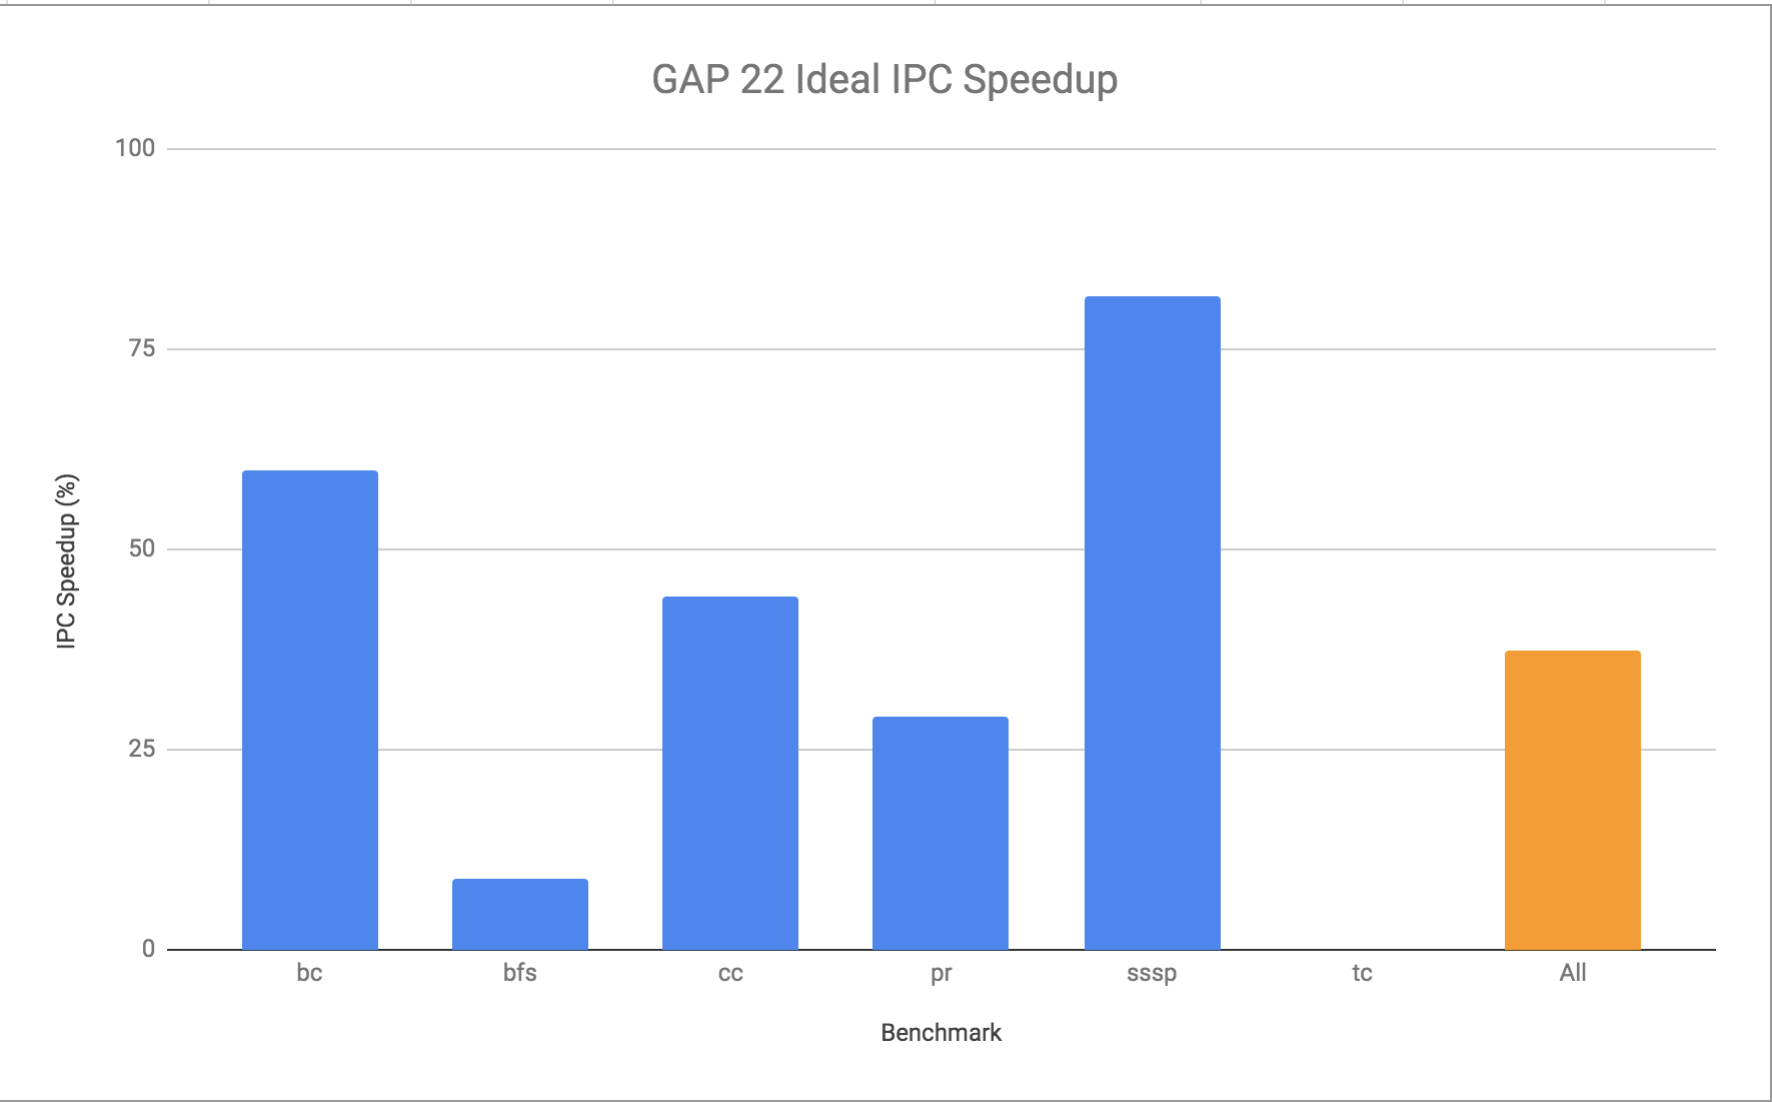
\includegraphics[width=.5\textwidth]{gap22_ideal}
        \caption{Ideal headroom for GAP-22 benchmarks}
    \end{figure}
 
    
    \subsection{Implementation Motivation}
        The research question we aim to address in this paper is whether previous intuition and methods used for cache line prefetching can be used to prefetch TLB translations. There are two key differences between cache line prefetching and TLB prefetching: the latency being hidden and the granularity of prefetches. Cache line prefetchers attempt to hide the latency of going to memory for data at a specific physical address, whereas the goal of TLB prefetching is to hide the latency of walking the page table for a translation from a virtual address to physical address. Additionally, the granularity at which prefetches cover the address space of a system is significantly larger for a TLB prefetcher than a cache line prefetcher. These key differences motivate the TLB prefetchers implemented in this paper. Section \ref{TAKEAWAYS} will discuss more on how page granularity affects the design and considerations of a prefetcher. 

\section{Implementations} \label{Implementation}
    \subsection{State of the Art - ``Delta''}
        The previous state of the art is Distance Prefetching proposed in \cite{c1}. Distance prefetching works by correlating the distance of the current page from the previous page to a list of $S$ slots, where each slot contains a correlated delta. These correlated deltas are then added to the current page to create predicted addresses. Our implementation of DP, which we refer to as “Delta”, trains the predictor on the total access stream.     
    \subsection{Global Address Correlation - ``GAC"}
        % RUSHI
        Traditional Global Address Correlation is well-explored in prefetching literature. We implemented the same Global Address Correlation (``GAC'') idea for TLB prefetching with a few key differences. For example, rather than correlating cache lines, we operate at the page granularity. So each page maintains a set of $S$ correlated pages trained on the total access stream. This set is managed on an LRU basis, and experiments were conducted with $S = 2$. When that page is seen again, its correlated set of pages is prefetched. 
        
    \subsection{PC Localized Address Correlation - ``PLAC"}
        % RUSHI
        We modified our GAC implementation slightly to localize based on the PC of the load instruction. So, for every unique PC we store a copy of the metadata we mentioned in the previous GAC section. Note that this is a standard approach in traditional prefetching literature. 

    \subsection{Footprinting Page Correlation}
        % RUSHI
        As a motivating example for this approach, consider $Page_A$ that holds $Data Structure_1$ in the first half of the page and holds $DataStructure_2$ in the second half of the page. Whenever the code accesses $DataStructure_1$ it will access $Page_B$ next. Similarly, whenever the code accesses $DataStructure_2$ it will access $Page_C$ next. Simply correlating $Page_A$ with only one of $Page_B, Page_C$ would be insufficient. Instead, we want to capture access information at a granularity that is finer than page granularity. 
        
        Thus, we correlate every page with a list of footprints in a metadata structure. These footprints represent the access pattern within a page. In turn, these footprints correlate to a page expected to follow that access stream. Footprints are snapshotted into the metadata structure on every access. Every access also updates the current footprint for the current page. Prefetches are issued every time the current footprint in a page is sufficiently similar to a snapshotted footprint for that page. This condition is checked on every access. The metadata stored is outlined in the attached schematic.
        
        \begin{figure}[h]
            \centering
                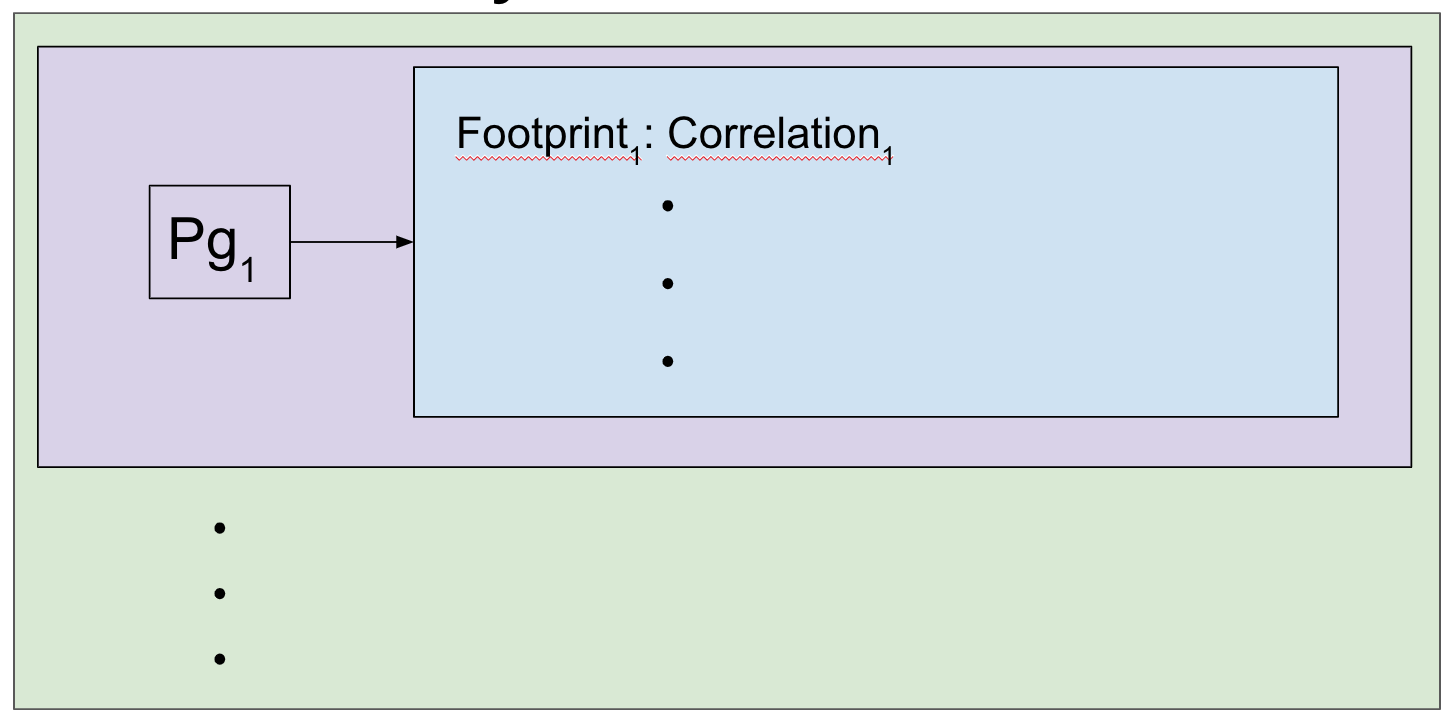
\includegraphics[width=.5\textwidth]{footprint_metadata.png}
            \caption{Footprint Page Correlation Data Structure}
        \end{figure}
        
        A page's footprint is represented as a bitset where each address in the page corresponds to one bit in the bitset. If this is too fine of a granularity, it can be made coarser by chunking up the addresses in a page, for example at the cache line granularity. 
        
        In the motivating example, the next time an access stream starts accessing $DataStructure_1$, the prefetcher will recognize the footprint as accessing primarily the first half of the page and issue a prefetch for $Page_B$.
        
        In our implementation, we somehow introduced an unidentifiable bug that stops the prefetcher from issuing any prefetches. Because we were not able to identify the bug in the implementation, we were not able to collect results for this prefetcher. 

    \subsection{Offset History}
        This prefetcher, shown in Figure~\ref{fig:offset} attempts to solve the same motivating example described above for Footprinting Page Correlation. 

        Offset history works by correlating a history of address access offsets within a page to a delta. This delta represents the predicted distance from the current page to prefetch a TLB translation. The offsets are not localized by page in the history vector. Instead, they are localized by PC to capture code flow of the program without enforcing specific page addresses. 

        This prefetcher addresses one of the short comings of the footprint based solution: the loss of ordering information. The offset history vector maintains the order in which a stream accesses data in pages. 

        We ran preliminary tests to determine the results of Offset History using SPEC 2006 and determined that it performs worse than PLAC and the baseline no prefetcher for many benchmarks, despite maintaining a high accuracy. Thus, we decided not to focus on this prefetcher for the remainder of this work. 

        \begin{figure}[h]
            \centering
                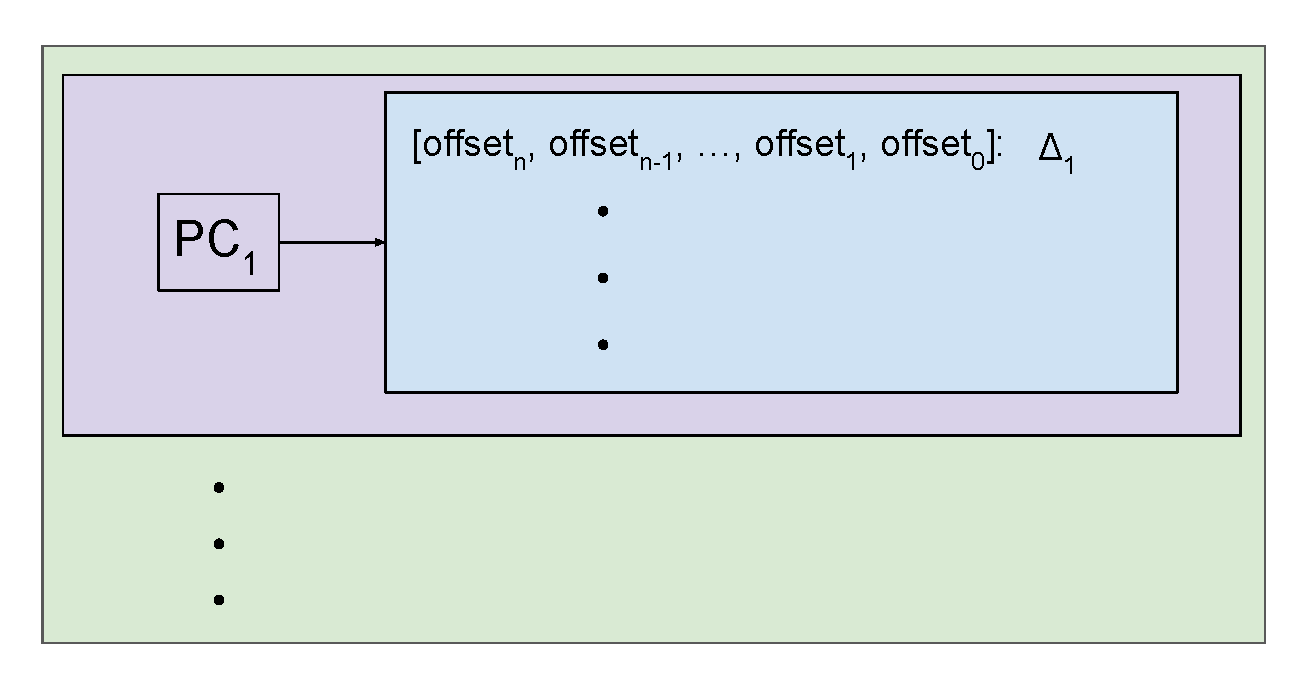
\includegraphics[width=.5\textwidth]{offset_history.pdf}
            \caption{Offset History Prefetcher data structure}
            \label{fig:offset}
        \end{figure}

    \begin{figure*}[p]
        \centering
            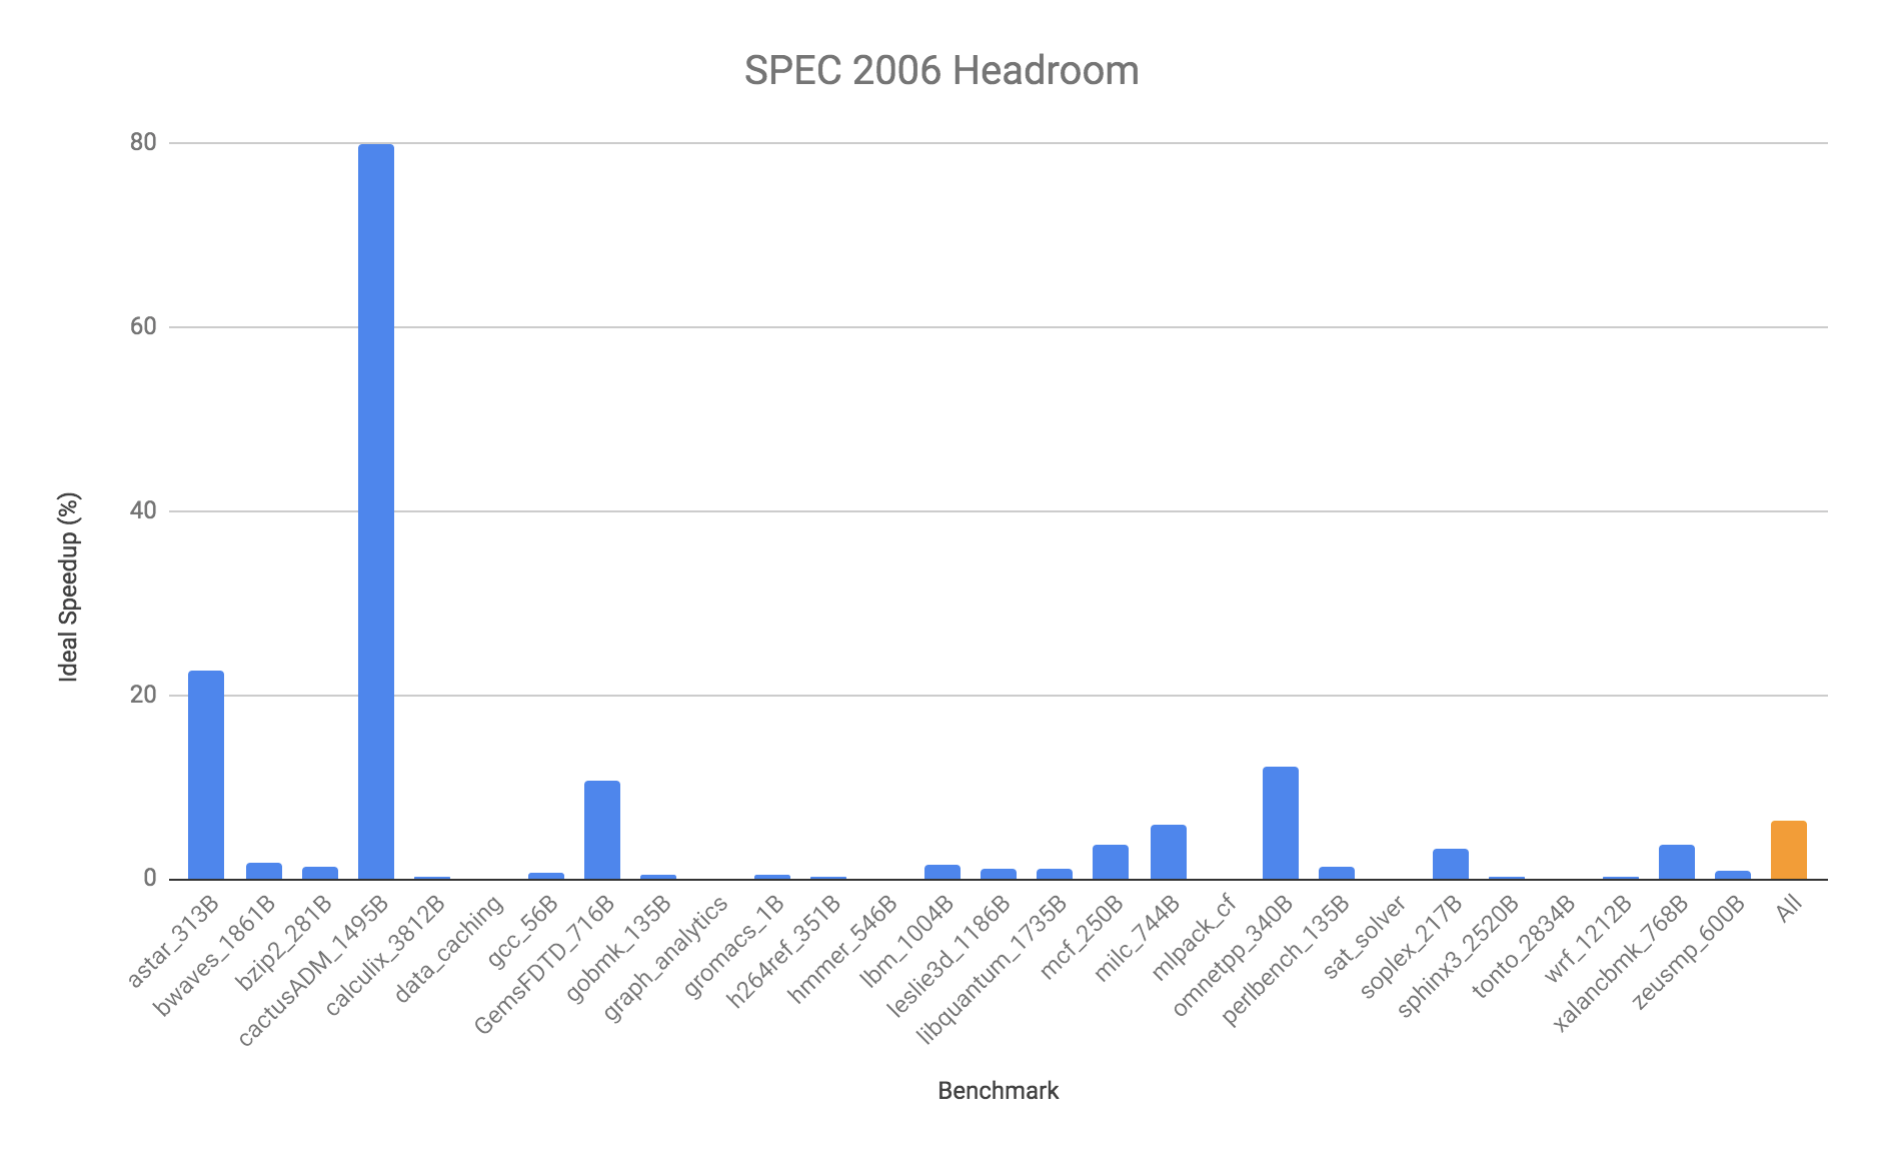
\includegraphics[width=.95\textwidth]{spec_ideal}
        \caption{Ideal headroom for SPEC 2006 benchmarks}
        \vspace*{\floatsep}
        \vspace*{\floatsep}
            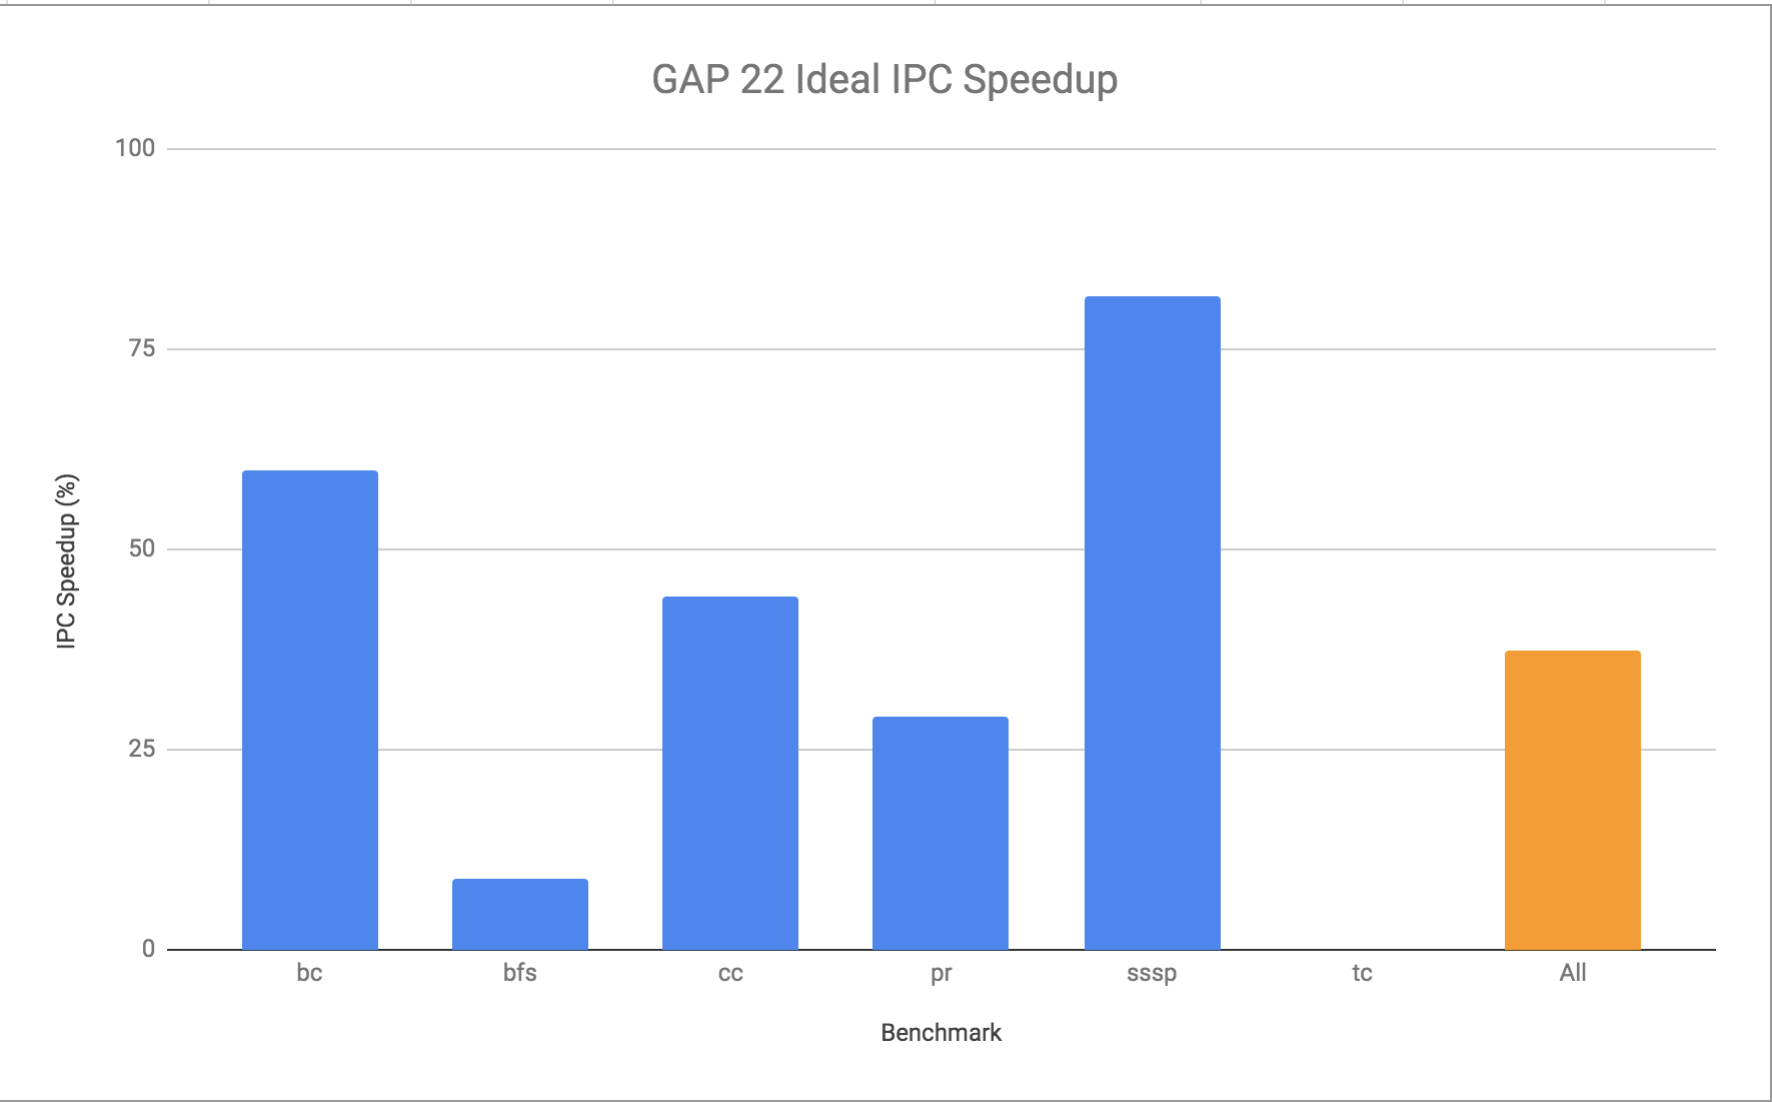
\includegraphics[width=.75\textwidth]{gap22_ideal}
        \caption{Ideal headroom for GAP-22 benchmarks}
    \end{figure*}
\section{Experimentation \& Results}

    \subsection{Headroom Study}
        % RUSHI
        The first experiment we conducted was a comprehensive headroom study in ChampSim to motivate further experimentation. We are presenting the results of the experiments on four benchmark suites: SPEC 2006, SPEC 2017, GAP 22, and Cloudsuite. We simulated an ideal TLB prefetcher by configuring ChampSim to treat any TLB access as zero-latency. We present the results of the speedup of IPC when compared to no prefetching and full-latency translation accesses. 

        GAP 22 had the most promising and realistic headroom results. Other than the \textbf{tc} benchmark, every benchmark in the GAP 22 suite had at least \textasciitilde{}9\% ideal speedup, with an average of 37.3\% speedup. 

        SPEC 2006 also had promising headroom results, particularly the \textbf{cactus} benchmark which had an ideal speedup of \textasciitilde{}80\%. The average ideal speedup was a respectable 6.4\%.

        SPEC 2017, however, looked underwhelming. It only had an average ideal speedup of 1.08\% and only one benchmark managed to break past a 10\% speedup over no prefetching. The Cloudsuite benchmark suite was a set of multicore programs. The initial headroom results looked unbelievably promising, with an average ideal speedup of over 260\%. However, no prefetcher was able to capture this insane headroom. We think further thought process needs to go into multicore benchmarks before results can be convincing. SPEC 2017 and Cloudsuite headroom graphs are reserved for the appendix.
    
    
    \subsection{General Results}

    A variety of workloads were run on ChampSim to determine the performance of our TLB prefetcher. In this case, our prefetchers were run SPEC 2006, GAP-22, and Cloudsuite workloads and were then analyzed based on IPC, coverage, redundancy, and prefetcher accuracy. 
    
    When we compare the overall prefetcher accuracy for SPEC 2006 (in Figure 11, Appendix) we observe that PLAC, for the most part, is able to dominate the other prefetchers, with an average accuracy of $\sim$30\% compared to Delta's 16\%. However, it's important to note that prefetcher accuracy is not representative of performance since there could be a high number of redundant prefetches (or not as many prefetches being issued.) We see similar results for GAP-22, but since this data is not significant, we will not include it.
    
    \begin{figure*}[h]
        \centering
            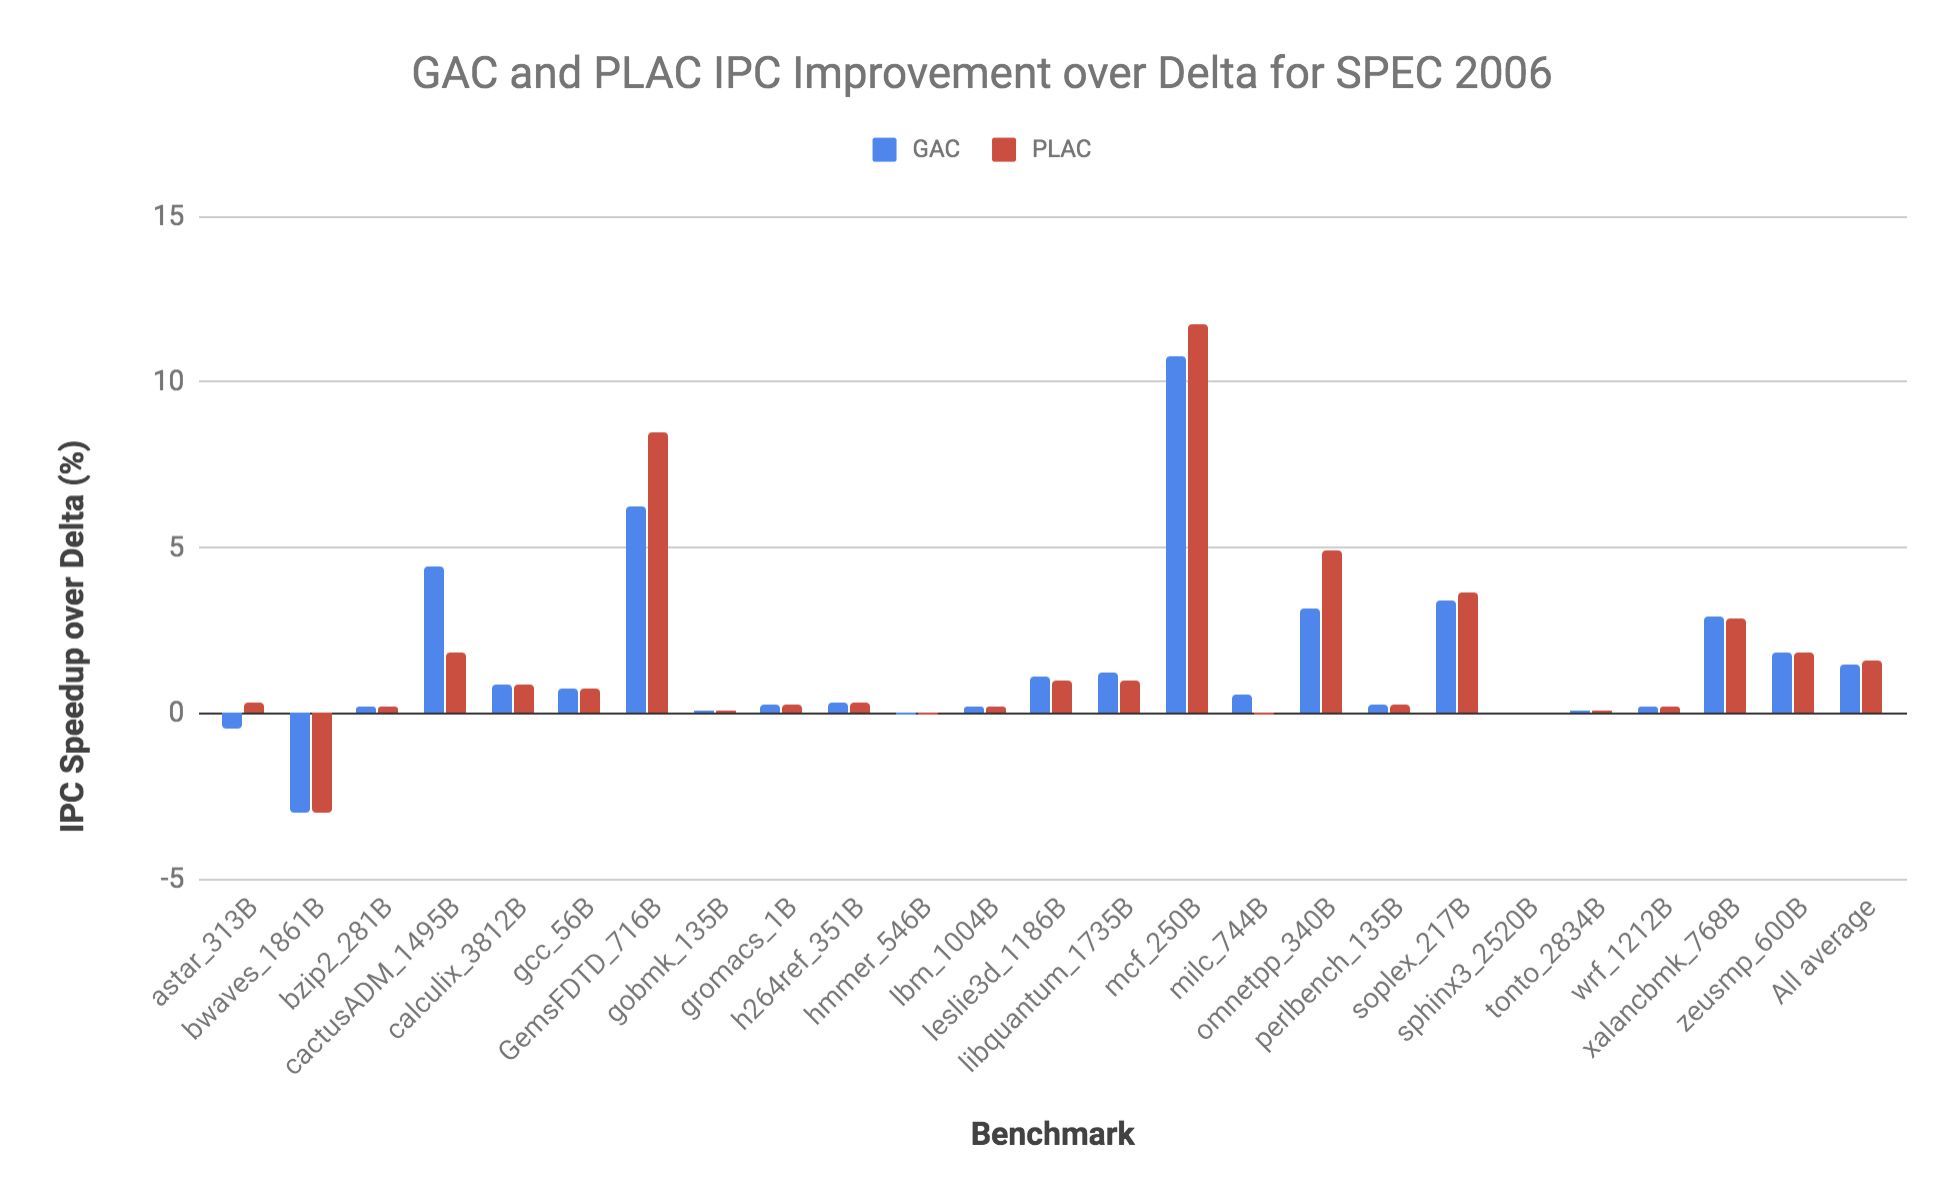
\includegraphics[width=.95\textwidth]{ipc_spec2006.png}
        \caption{SPEC 2006 IPC improvement over Delta}
    \end{figure*}
    
     Looking at prefetcher redundancy for SPEC 2006 (in Figure 12, Appendix), we clearly see that both GAC and PLAC issue a significantly larger number of prefetches compared to the delta prefetcher. On average, PLAC issues prefetches at 79\% redudancy, where as Delta has a redundancy rate of 63\%. The main conclusion here is that our prefetcher is not issuing any useful requests to memory to save memory latency. When we take a look at the GAP 22 benchmarks (in figure 17, Appendix), we see a similar result of low redundancy for Delta (at around 29\%) compared to GAC and PLAC, which had 49\% and 52\% redundancy respectively. 
     
    Since performance can be mostly quantified with the IPC, we want to focus on the IPC improvement over Delta for SPEC 2006 benchmarks and GAP-22 (figure 6 and 8). We observe that for both GAC and PLAC, we have an average speed up over Delta at around 1.5\% (IPC improvement). An important takeaway from this data is that we observe significant gains in performance namely in benchmarks \textbf{GemsFDTD} and \textbf{mcf}. For GAP 22 (figure 8), we see that we see roughly 2-3\% IPC increase over Delta for both GAC and PLAC. Although the improvements are marginal, we observe visible gains that give further insights on the benefits of adding PC-granularity.

    Next we took a look at how much headroom our prefetchers captured in comparison to the Delta prefetcher. In this case, we specifically focused only on PLAC since it was our most promising prefetcher. We see that in the results for both GAP 22 and SPEC 2006 (figure 7, and 16 in the appendix), there is only marginal improvement compared to the Delta prefetcher. This can be attributed to the low coverage of GAC and PLAC, covering 15\% and 16\% of standard misses on the SPEC 2006 workloads. We observe that Delta's ability to cover compulsory misses allows it to have a much higher coverage for this suite.  We discuss later on how we can increase coverage. On the other hand, we observe that for the GAP-22 workloads (figure 19, appendix), PLAC has a coverage of 34\% compared to 28\% from Delta. One reason could be that the graph workloads could have more address correlation than anticipated. That, coupled with larger graph sizes, could amplify the effect of increased coverage. 
    
    \begin{figure}[h]
        \centering
            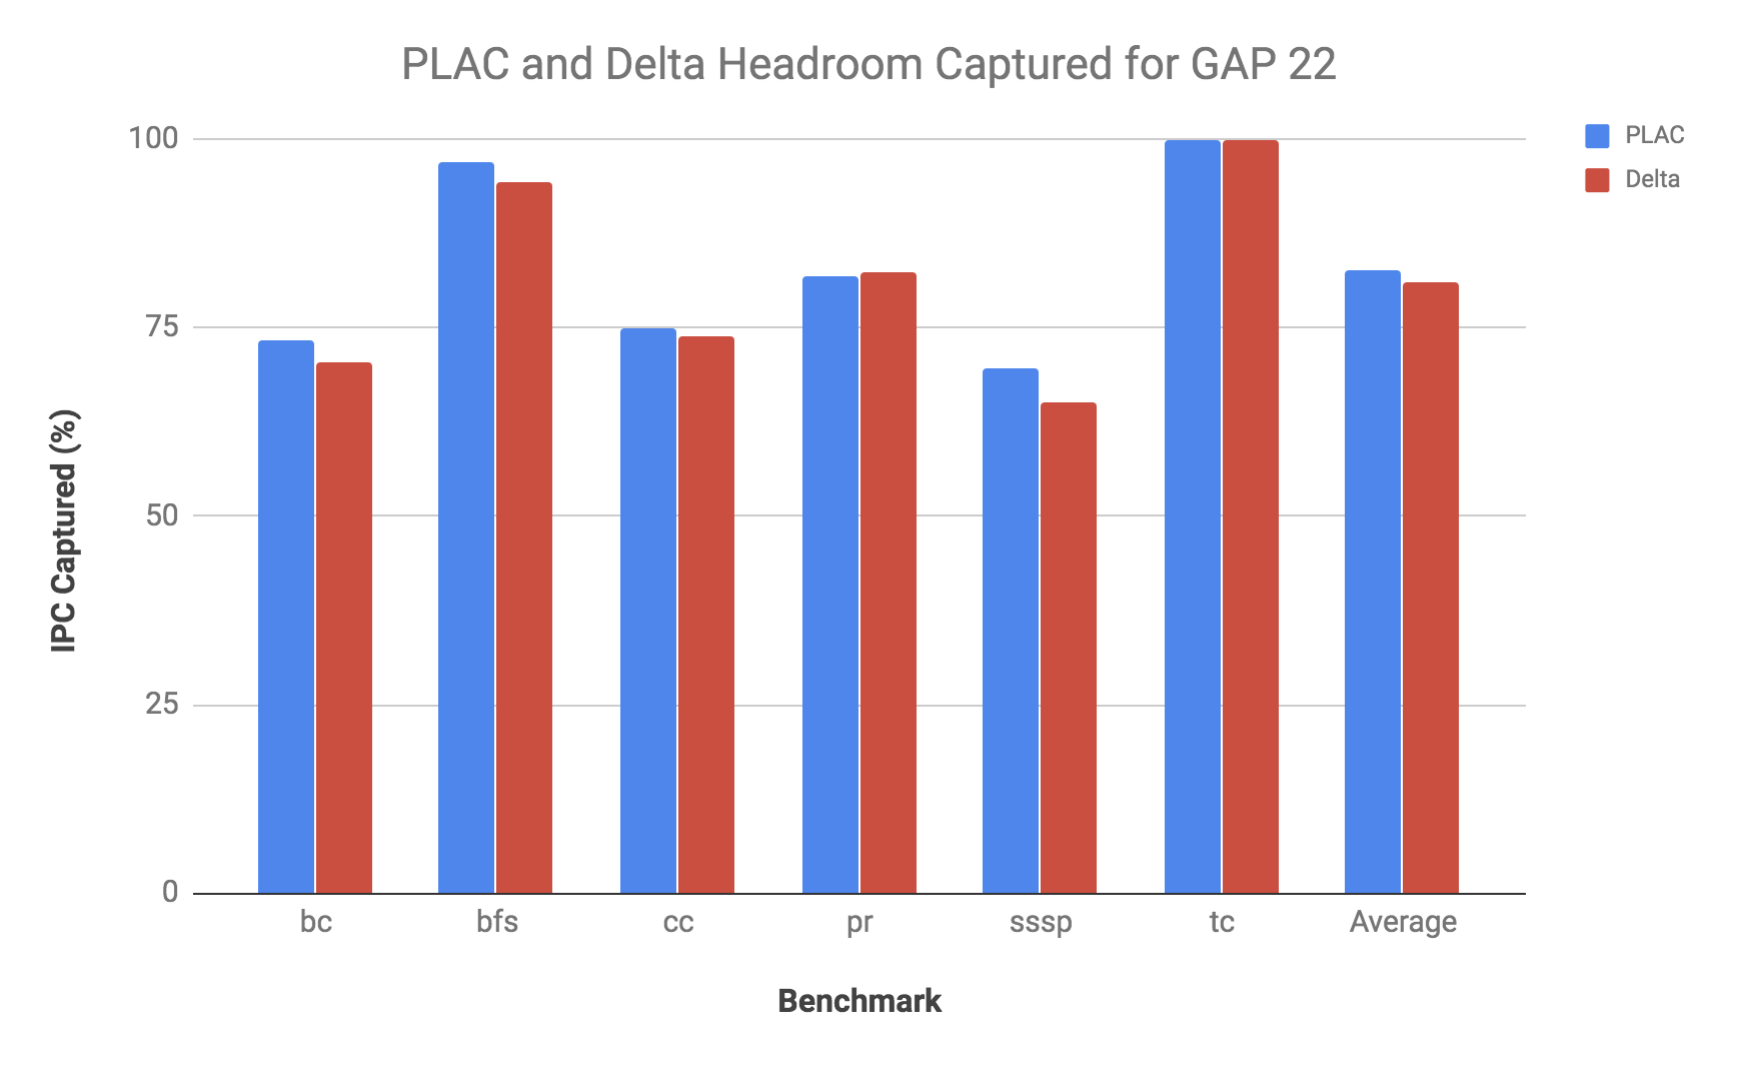
\includegraphics[width=.5\textwidth]{gap_covered.png}
        \caption{Headroom captured for GAP-22}
    \end{figure}

    \begin{figure*}[h]
        \centering
            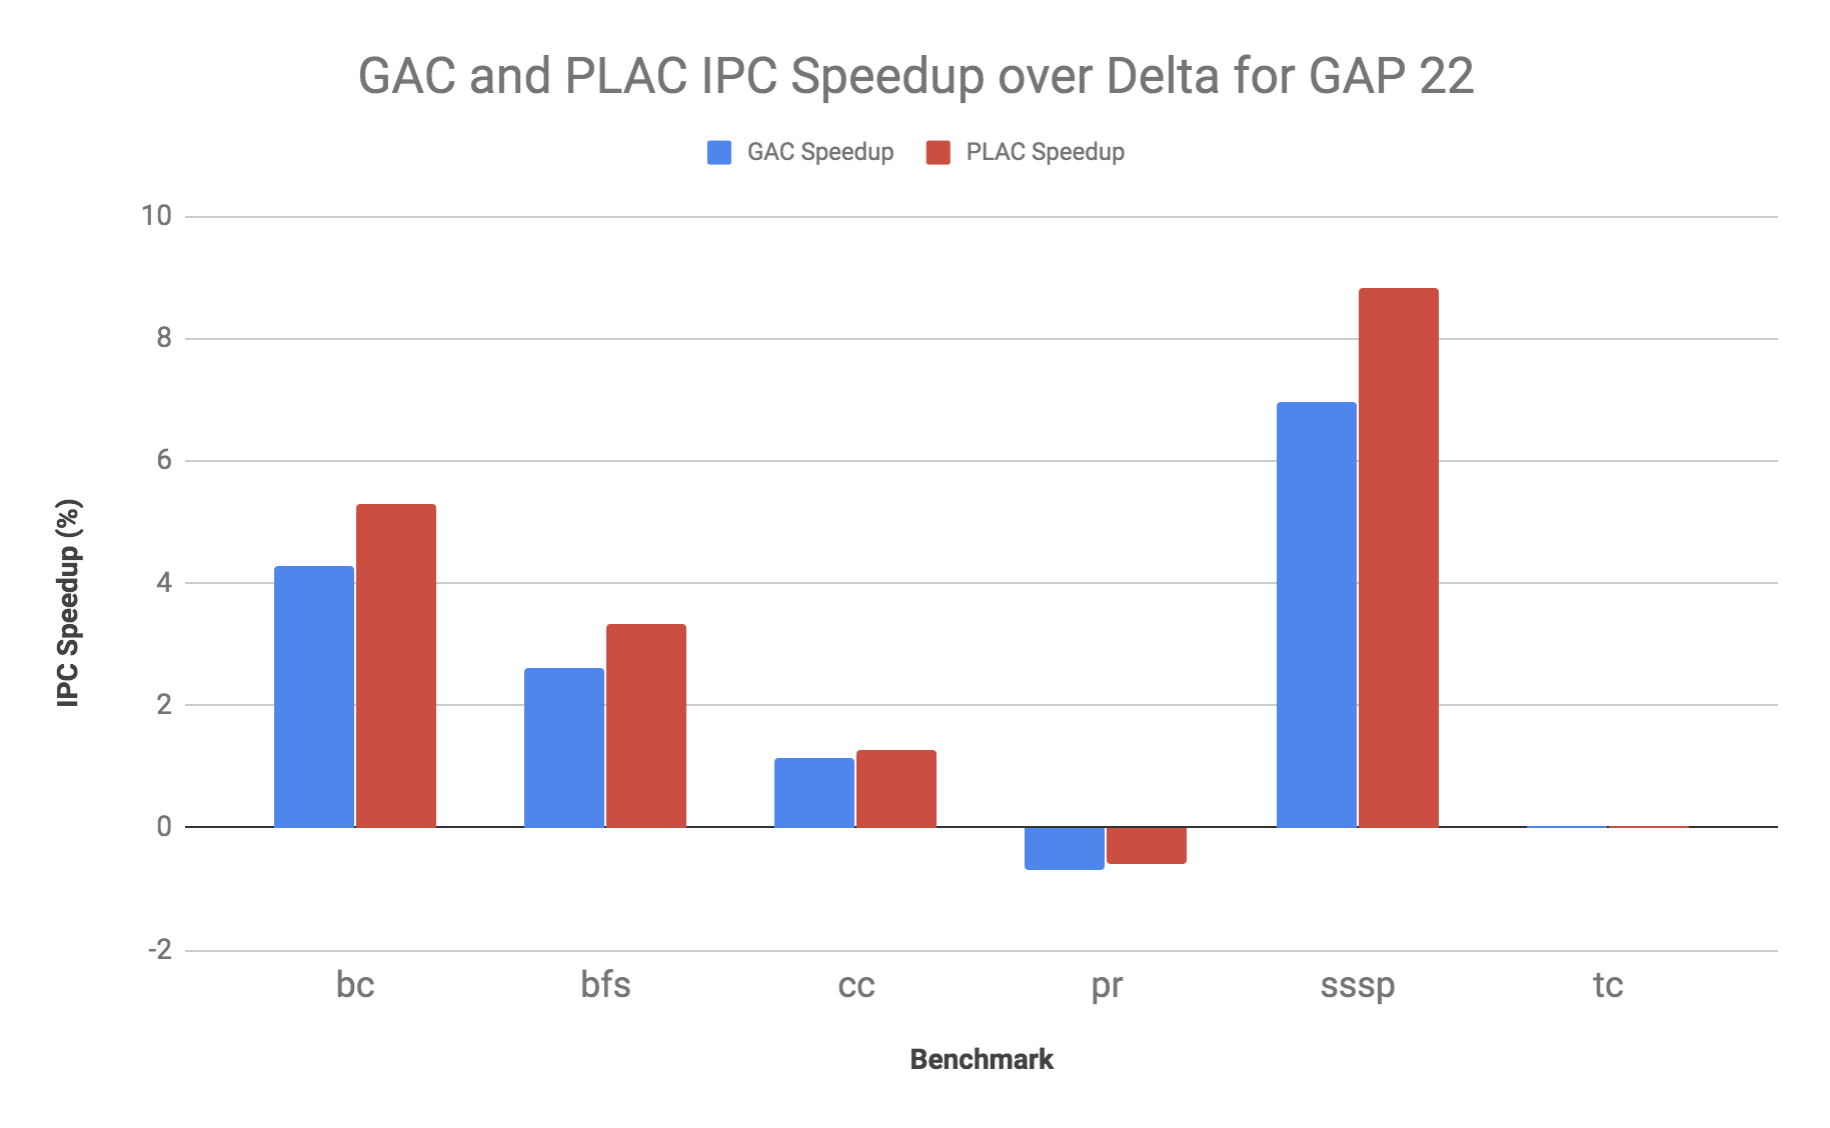
\includegraphics[width=.85\textwidth]{gac_plac_gap22.png}
        \caption{GAP-22 IPC speedup}
        \label{fig:gac_plac_speedup}
    \end{figure*}
    
    \subsection{Divergence Study}
        As mentioned in section~\ref{Implementation}, our implementations for Delta, GAC, and PLAC use a slot size of $S = 2$. The previous state of the art, \cite{c1}, found this slot size to be the optimal number of correlated deltas to a tag. To evaluate the amount of pages a given page can be correlated with in a program, we conducted a divergence study. This study simply counts the number of pages that immediately follow a page during execution. We ran this experiment for both GAP 22 and SPEC 2006. The results of our experiment are in figure~\ref{fig:g22_divergence} and \ref{fig:spec_divergence}. The y axis represents the average number of correlated pages for 99\% of pages in the indicated benchmark. Figure~\ref{fig:g22_divergence} shows that 99\% of pages in Gap-22 have an average of 6 correlated pages. Figure~\ref{fig:spec_divergence} shows that 99\% of pages in SPEC 2006 have an average of around 9 correlated pages. This figure also shows the high variability that exists between certain benchmarks. These graphs indicate that our prefetchers may benefit from increasing the slot size $S$. This may allow for higher predictor accuracy and improved performance.
        
        % Do we want to mention difference between average and max implies notable outliers? 
        
    \begin{figure}[h]
        \centering
            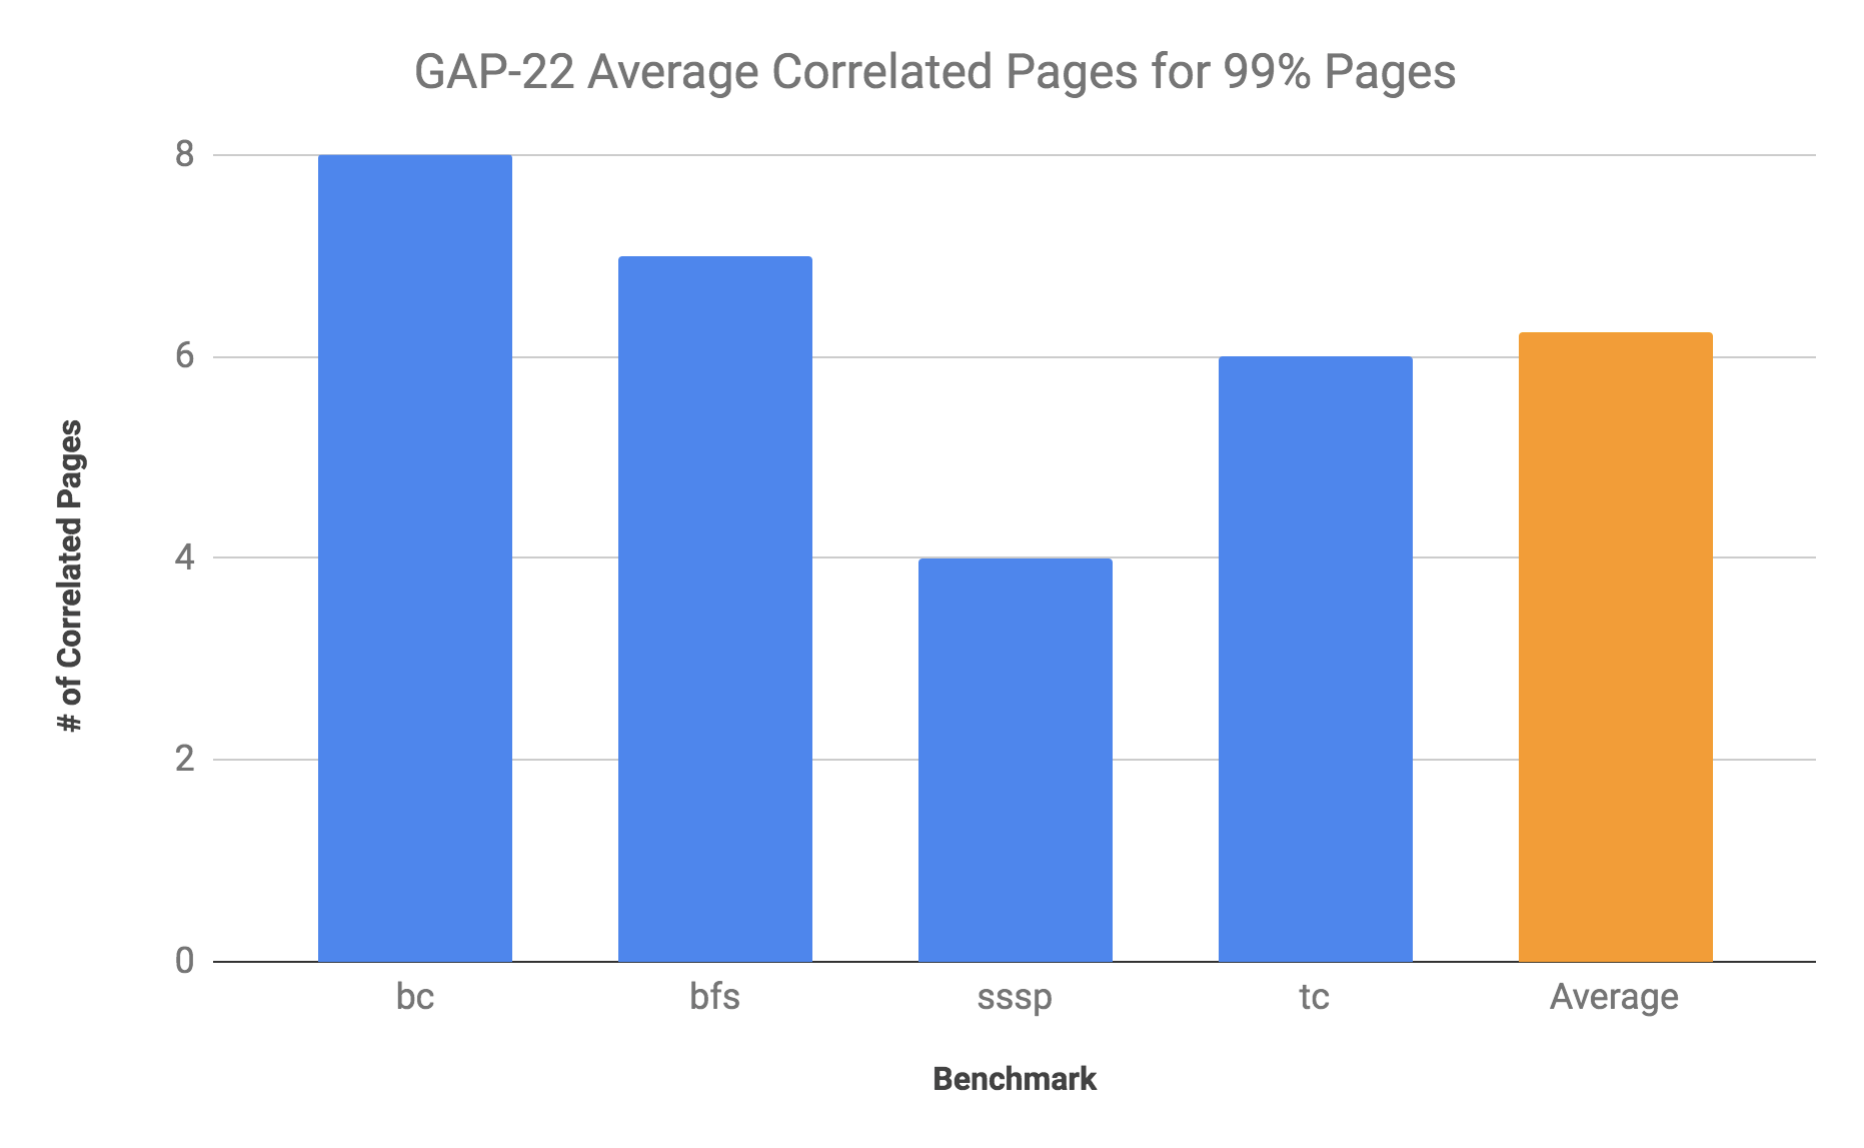
\includegraphics[width=.5\textwidth]{gap22_divergence_avg.png}
        \caption{Gap-22 Divergence Results}
        \label{fig:g22_divergence}
    \end{figure}
    
    %TODO: put spec image in
    \begin{figure}[h]
        \centering
            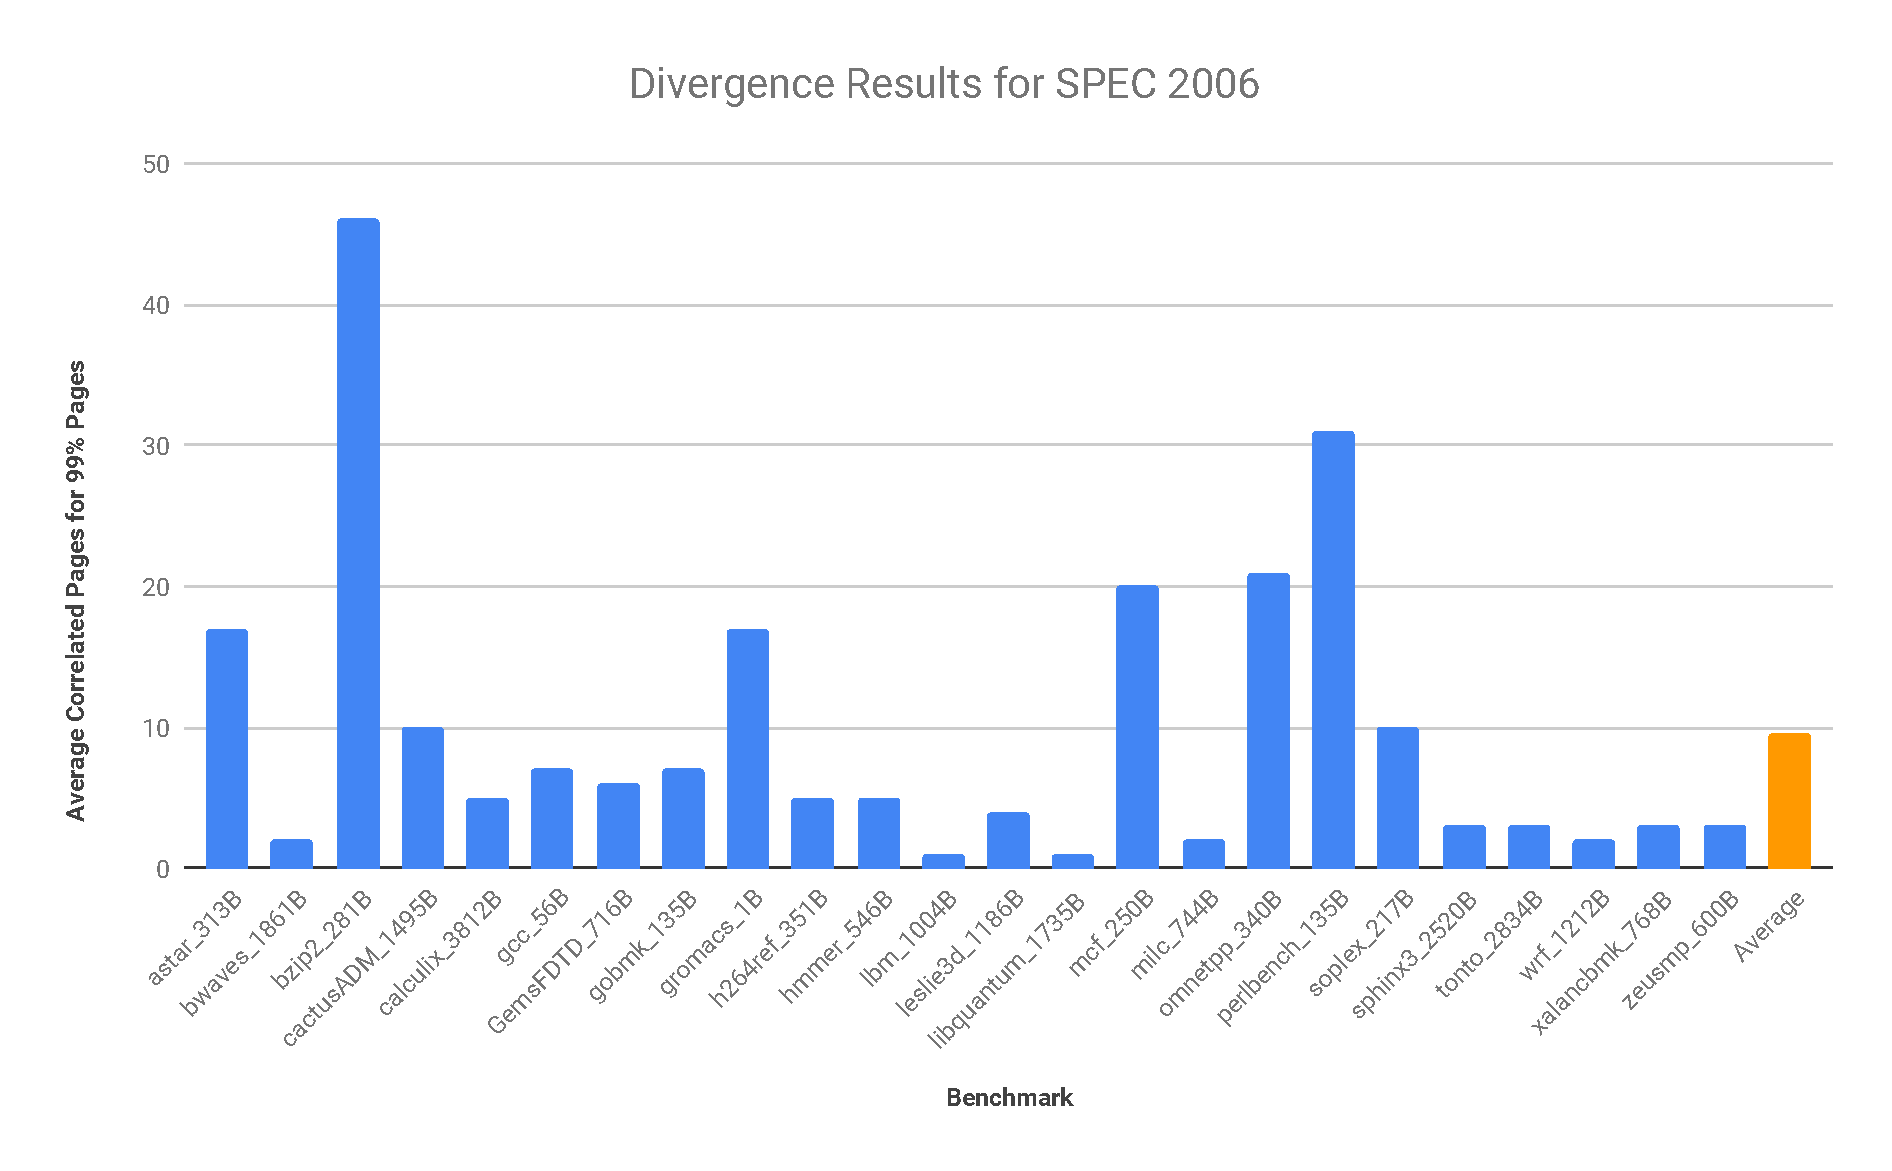
\includegraphics[width=.5\textwidth]{spec_divergence.pdf}
        \caption{SPEC 2006 Divergence Results}
        \label{fig:spec_divergence}
    \end{figure}

\section{TAKEAWAYS} \label{TAKEAWAYS}
    In this section, we provide high level takeaways from our study of TLB prefetchers.
    \subsection{Page Granularity}
        A key consideration when designing prefetchers is how data is laid out within a page. Given the size of a page, typically 4096 bytes, it may contain data for various different data structures. This can be seen in figure~\ref{fig:page_ds}. How these data structures are allocated within the page is a function of the memory allocation of the system and cannot be predicted for general programs, as programmers may allocate memory in non optimal ways or the OS may attempt to optimize memory layout. The TLB translation that is needed next may be tied to the specific data addresses accessed within a given period of time in a page. For example, if a program is accessing the tree data structure in the beginning of the page represented in figure~\ref{fig:page_ds}, it may next need the TLB translation for page B. However, if the program is accessing the linked list data structure in the lower end of the addresses of the figure, it may next need the TLB translation for page C. Given this insight and the results of the divergence study discussed in section~\ref{Implementation}, we recommend that future TLB prefetchers target divergence by using accesses within a page to capture the code flow of a program to determine page translations to prefetch. 
        
        This discussion leads to the next difficulty with page granularity prefetching for the TLB. In cache line prefetches, the triggering event is simply an access to a cache line. This is effective because when accessing a given cache line, the program will either reaccess that cache line or immediately move onto another cache line. However, at the page granularity, the system doesn’t know when the program will switch from accessing a given page to another. The system may make several accesses to a given page before switching, or may only make one. This again, is a result of the data layout within a page. This is an issue because, as discussed above, the prefetcher should maintain information on what addresses are accessed within a page. With this, there is no intuitive time in which the prefetcher has built up enough information on what data structures are being accessed within a page before issuing an educated prefetch. Therefore, more experimentation and research is necessary to determine what the optimal time to issue a TLB prefetch is. Our current work prefetches on every access to a page. However, we believe this can be improved to avoid TLB pollution and pressure.
            \begin{figure}[h]
            \vspace*{\floatsep}
            \centering
            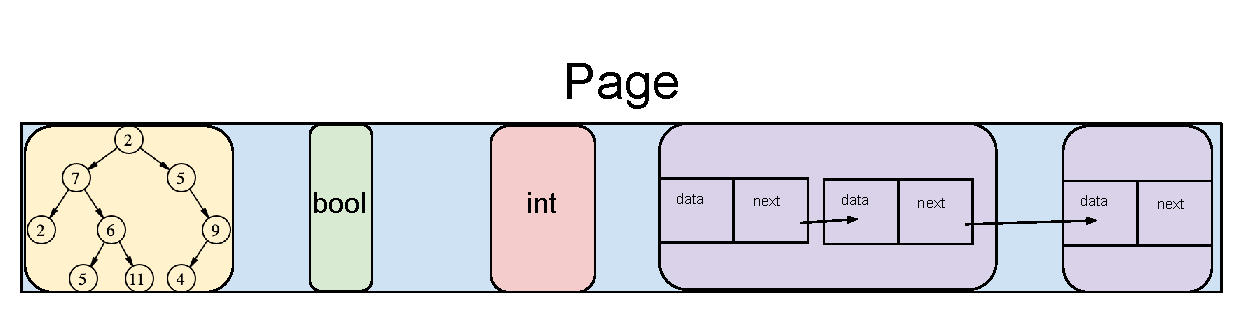
\includegraphics[width=.5\textwidth]{Page_granularity_data_structures.pdf}
            \caption{Data layout in a page}
            \label{fig:page_ds}
            \end{figure}
    \subsection{PC information}
        Given the previous discussion about the consideration of page granularity in the design of TLB prefetchers, information on the code flow of a program is necessary in order to gain information about how a given page is currently being accessed. One way to capture the code flow of a program is by using the program counter (PC) to localize a given stream of addresses. This is supported by our results for GAC and PLAC, where PLAC outperforms GAC, shown in figure~\ref{fig:gac_plac_speedup}.  
\section{FUTURE WORK}
    \subsubsection{Higher-degree prefetchers}
    As seen in the analysis of our results, low coverage and high redundancy were problems that drastically reduced the effectiveness of GAC and PLAC. By adjusting the degree of the prefetchers, effectively issuing more prefetches, we can attempt to reduce redundancy, and in turn, hope to increase coverage.
    
    \subsubsection{Hybrid prefetchers}
    Another potential idea would be to make use of a hybrid prefetcher to get the best of both worlds. A potential idea could be a PC/Delta prefetcher that could adjust according to the workload. This would improve the coverage as well as attempt to deliver the the IPC gains of PLAC.

\addtolength{\textheight}{-12cm}   % formatting something something, don't delete probably

\section*{APPENDIX}

    See attached graphs. % RUSHI

    \begin{figure*}[h] % RUSHI
        \centering
            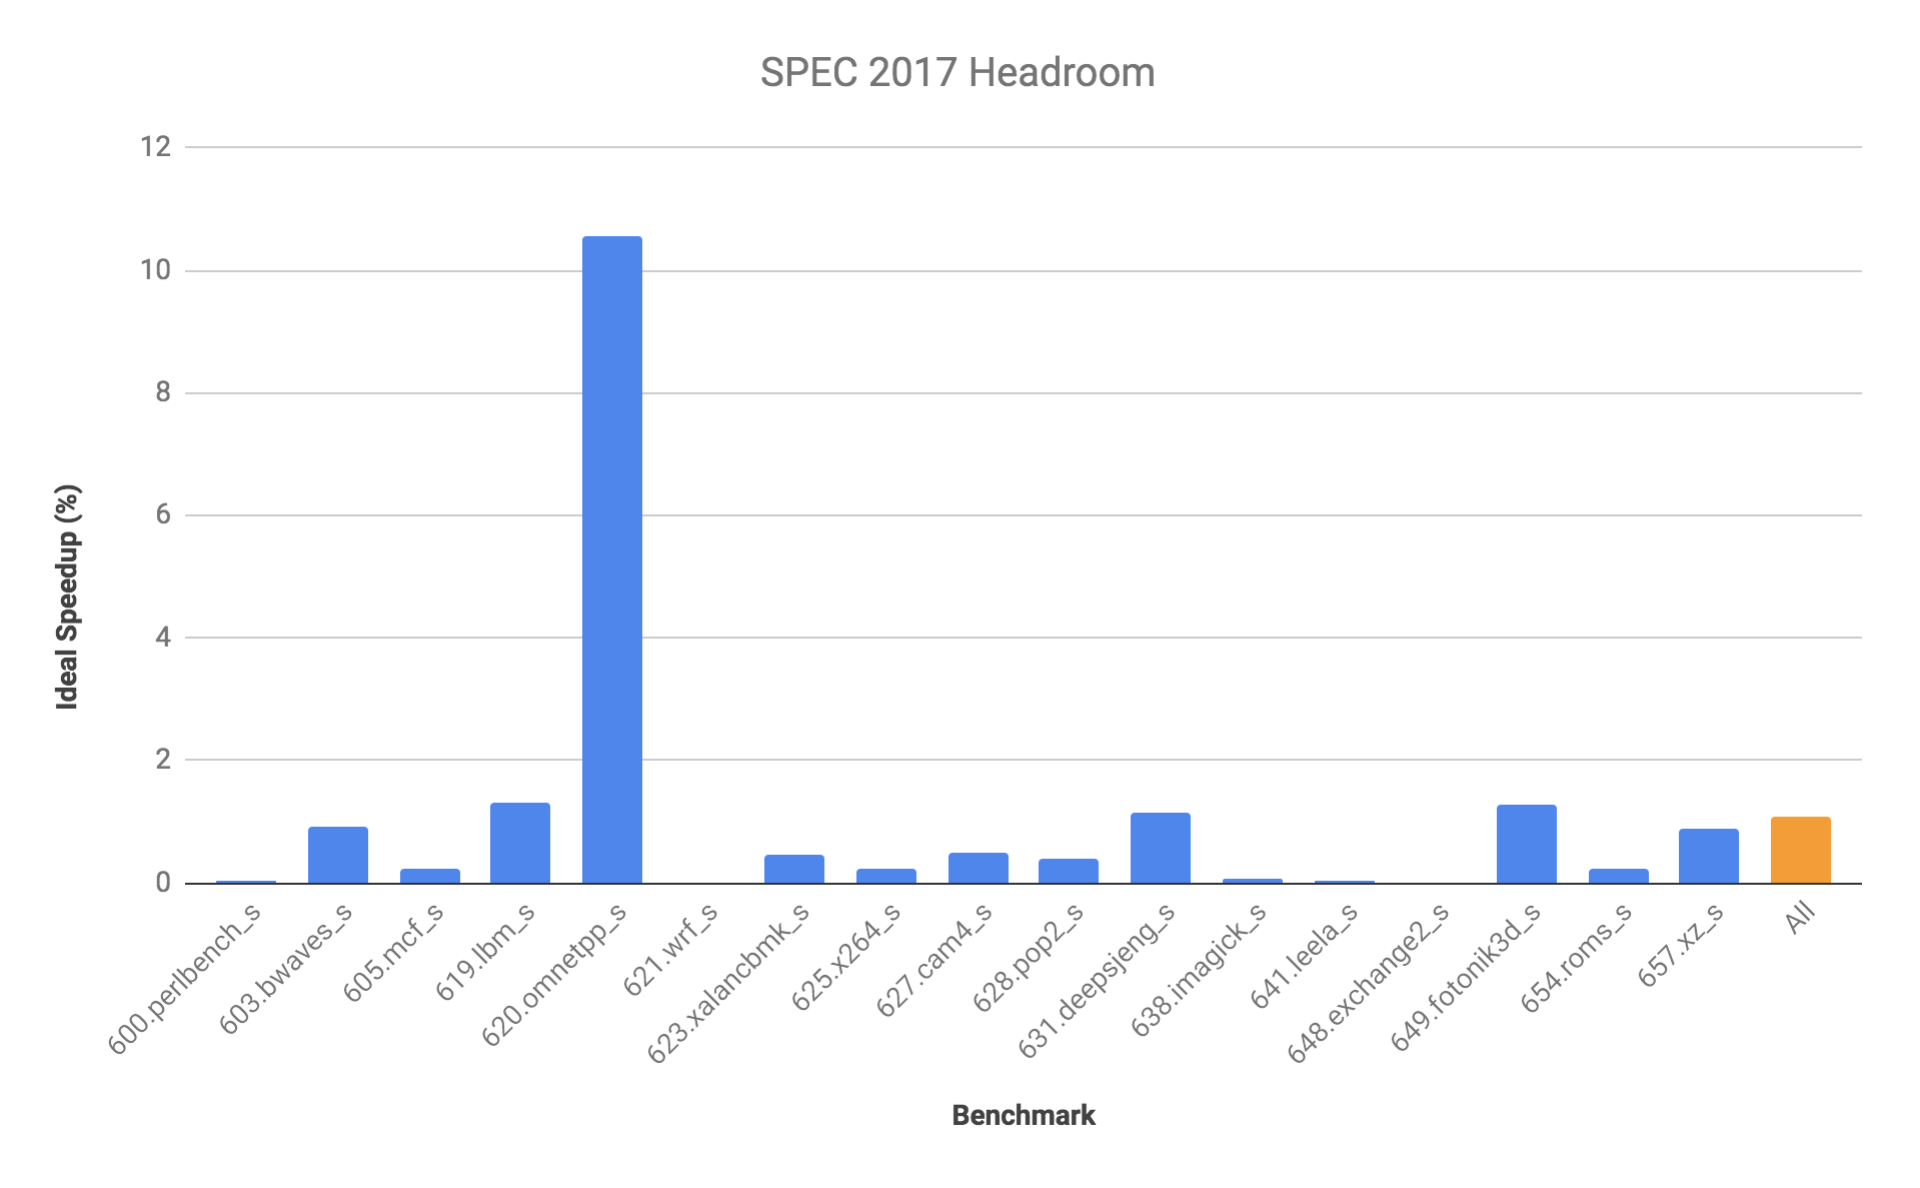
\includegraphics[width=.95\textwidth]{spec2017_ideal.png}
        \caption{Ideal headroom for SPEC 2017 benchmarks}
        \vspace*{\floatsep}
        \vspace*{\floatsep}
            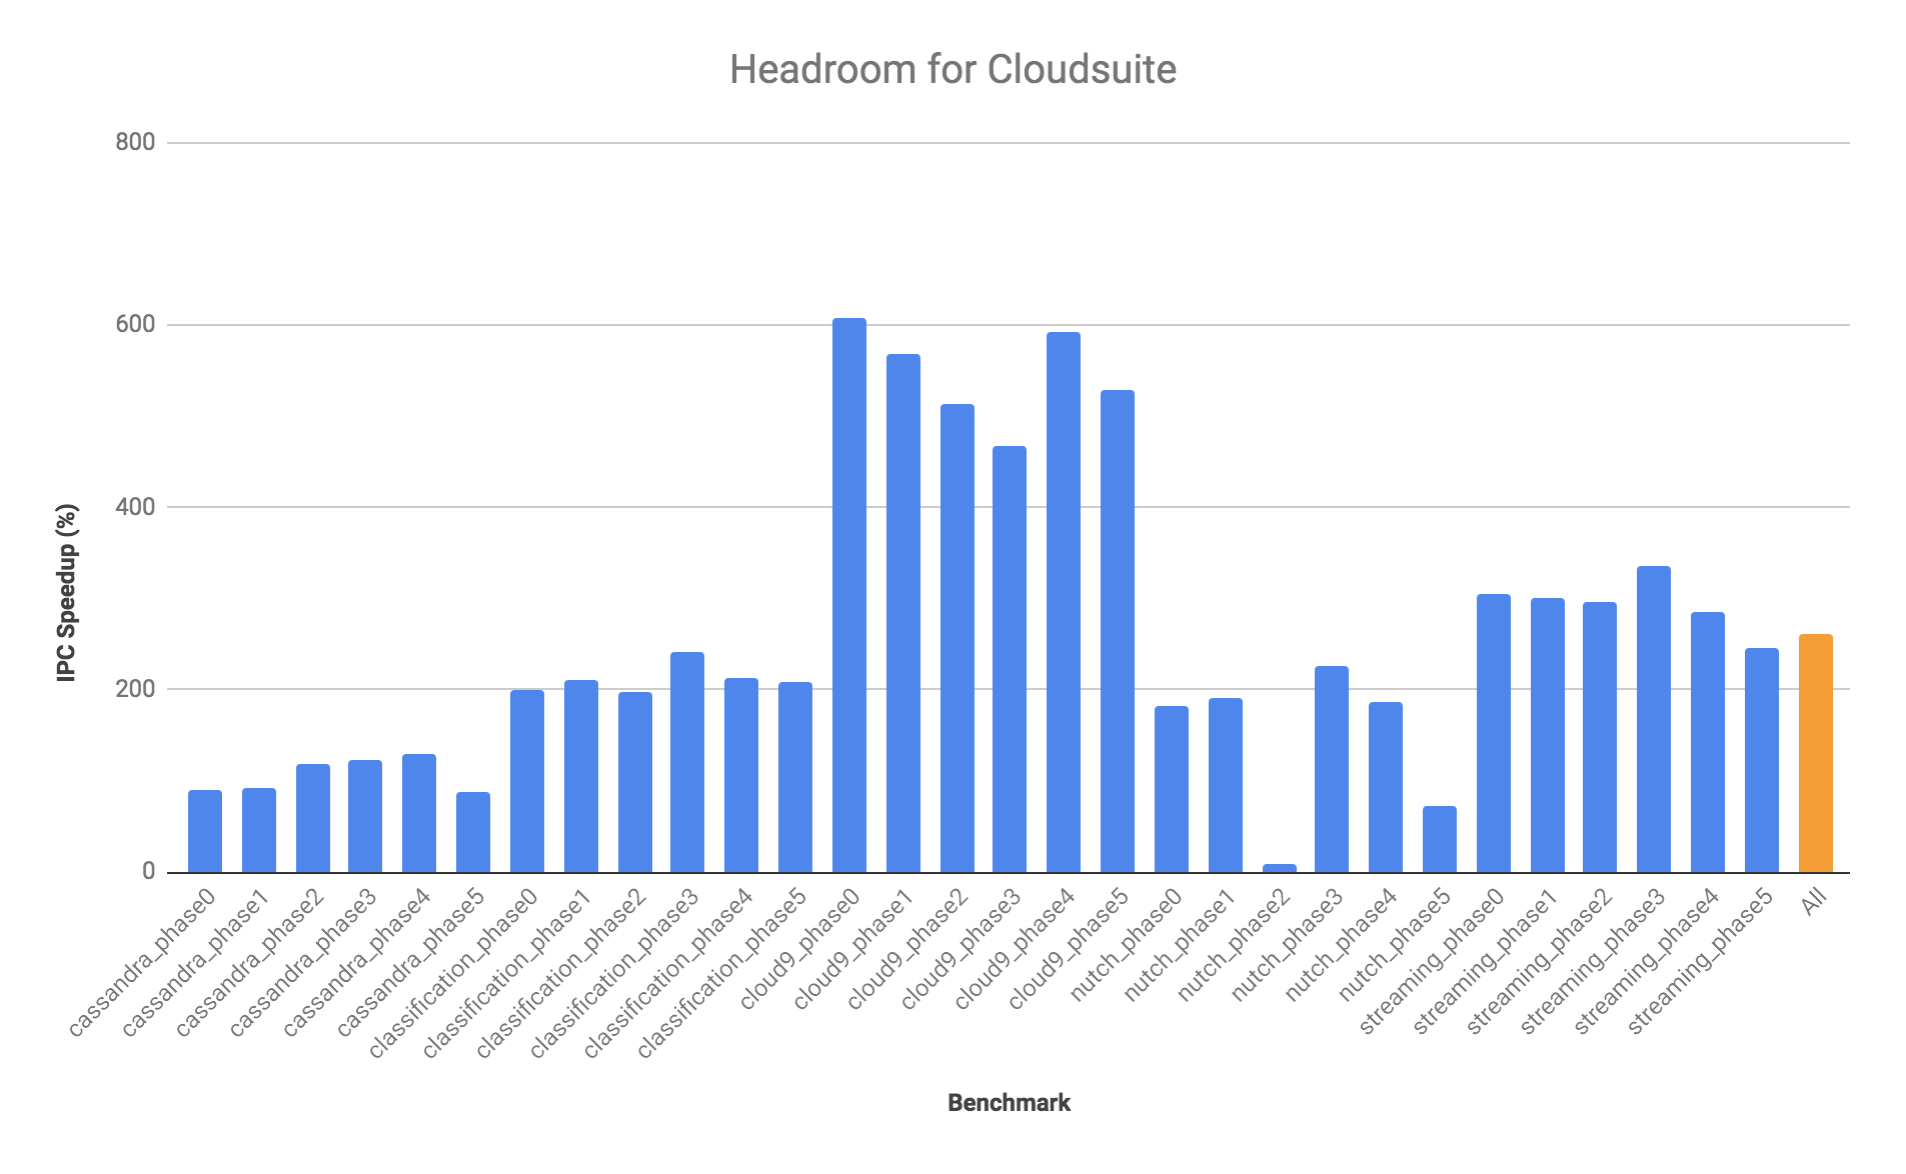
\includegraphics[width=.75\textwidth]{cloudsuite_ideal.png}
        \caption{Ideal headroom for Cloudsuite benchmarks}
    \end{figure*}
    
    \begin{figure*}[h] % RUSHI
        \centering
            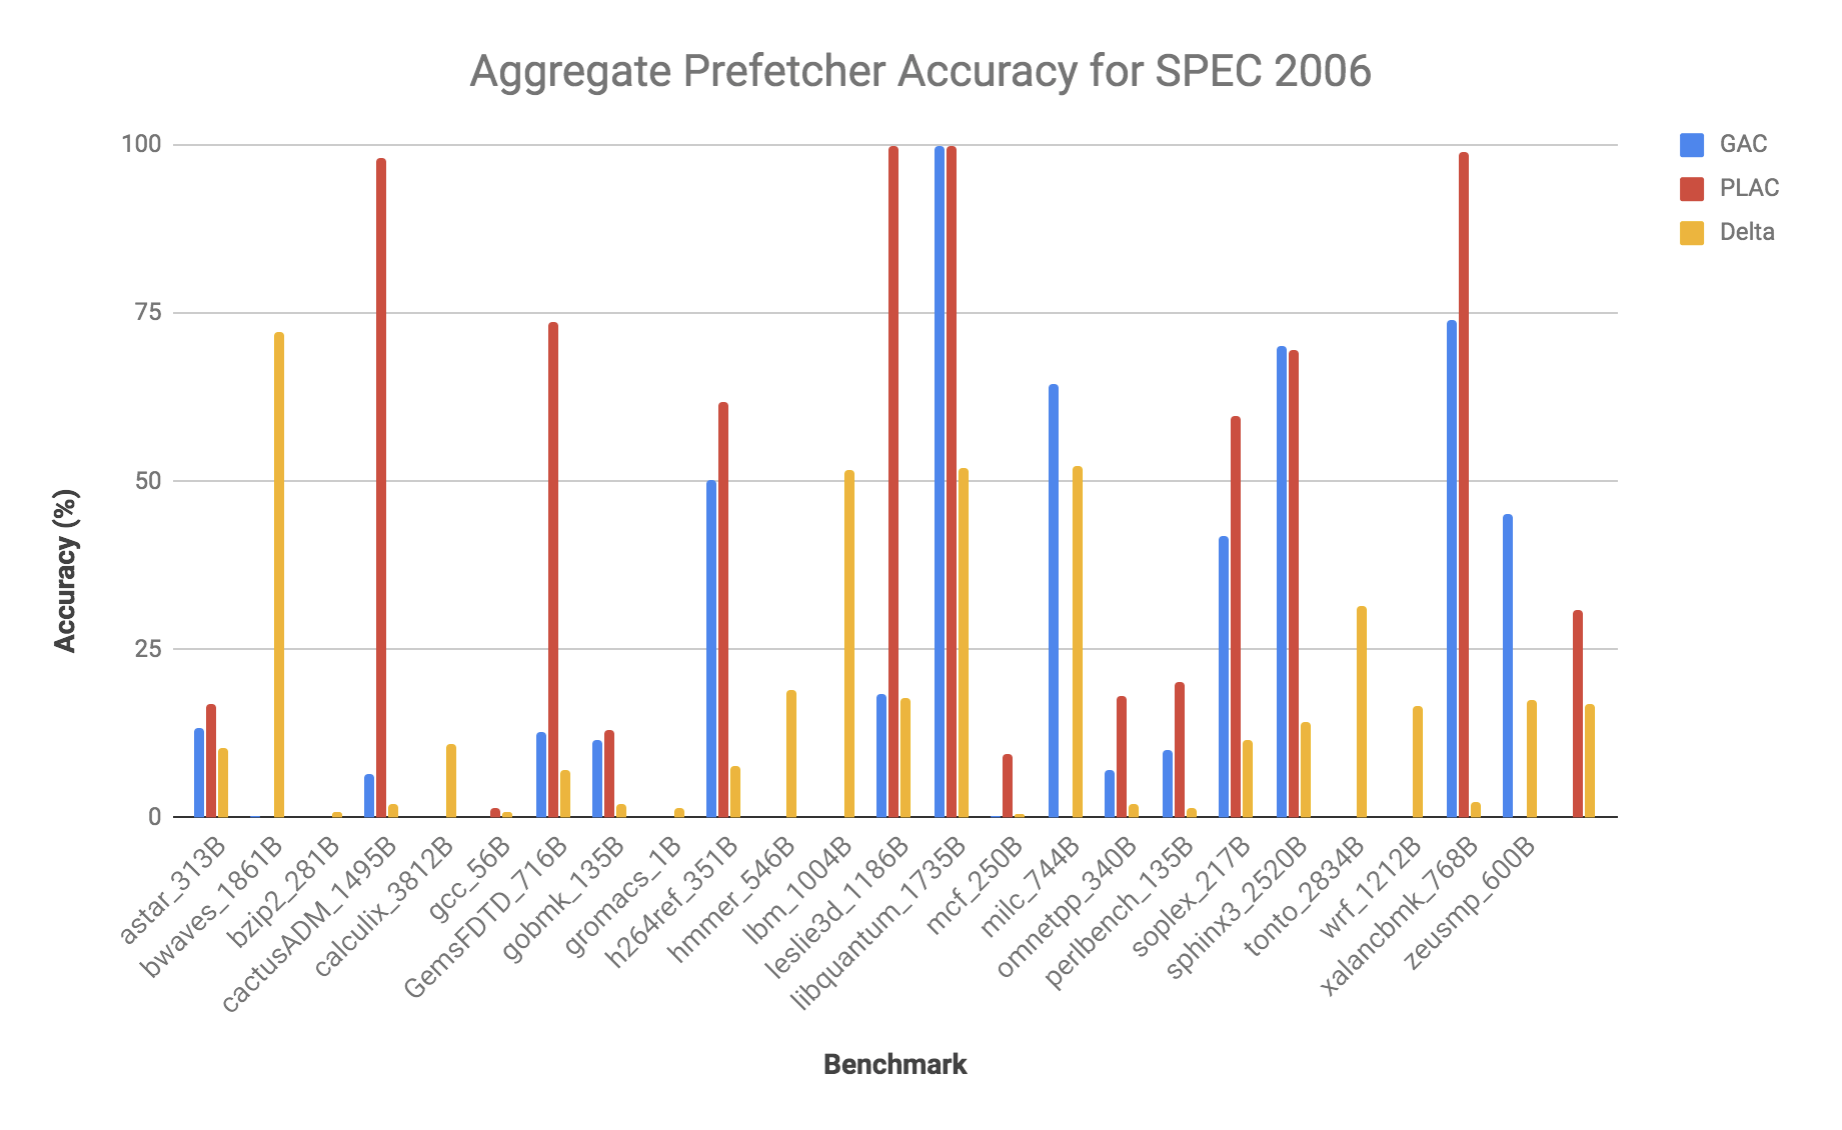
\includegraphics[width=.95\textwidth]{aggregate_accuracy.png}
        \caption{Prefetcher accuracy for SPEC 2006 benchmarks}
        \vspace*{\floatsep}
        \vspace*{\floatsep}
        \centering
            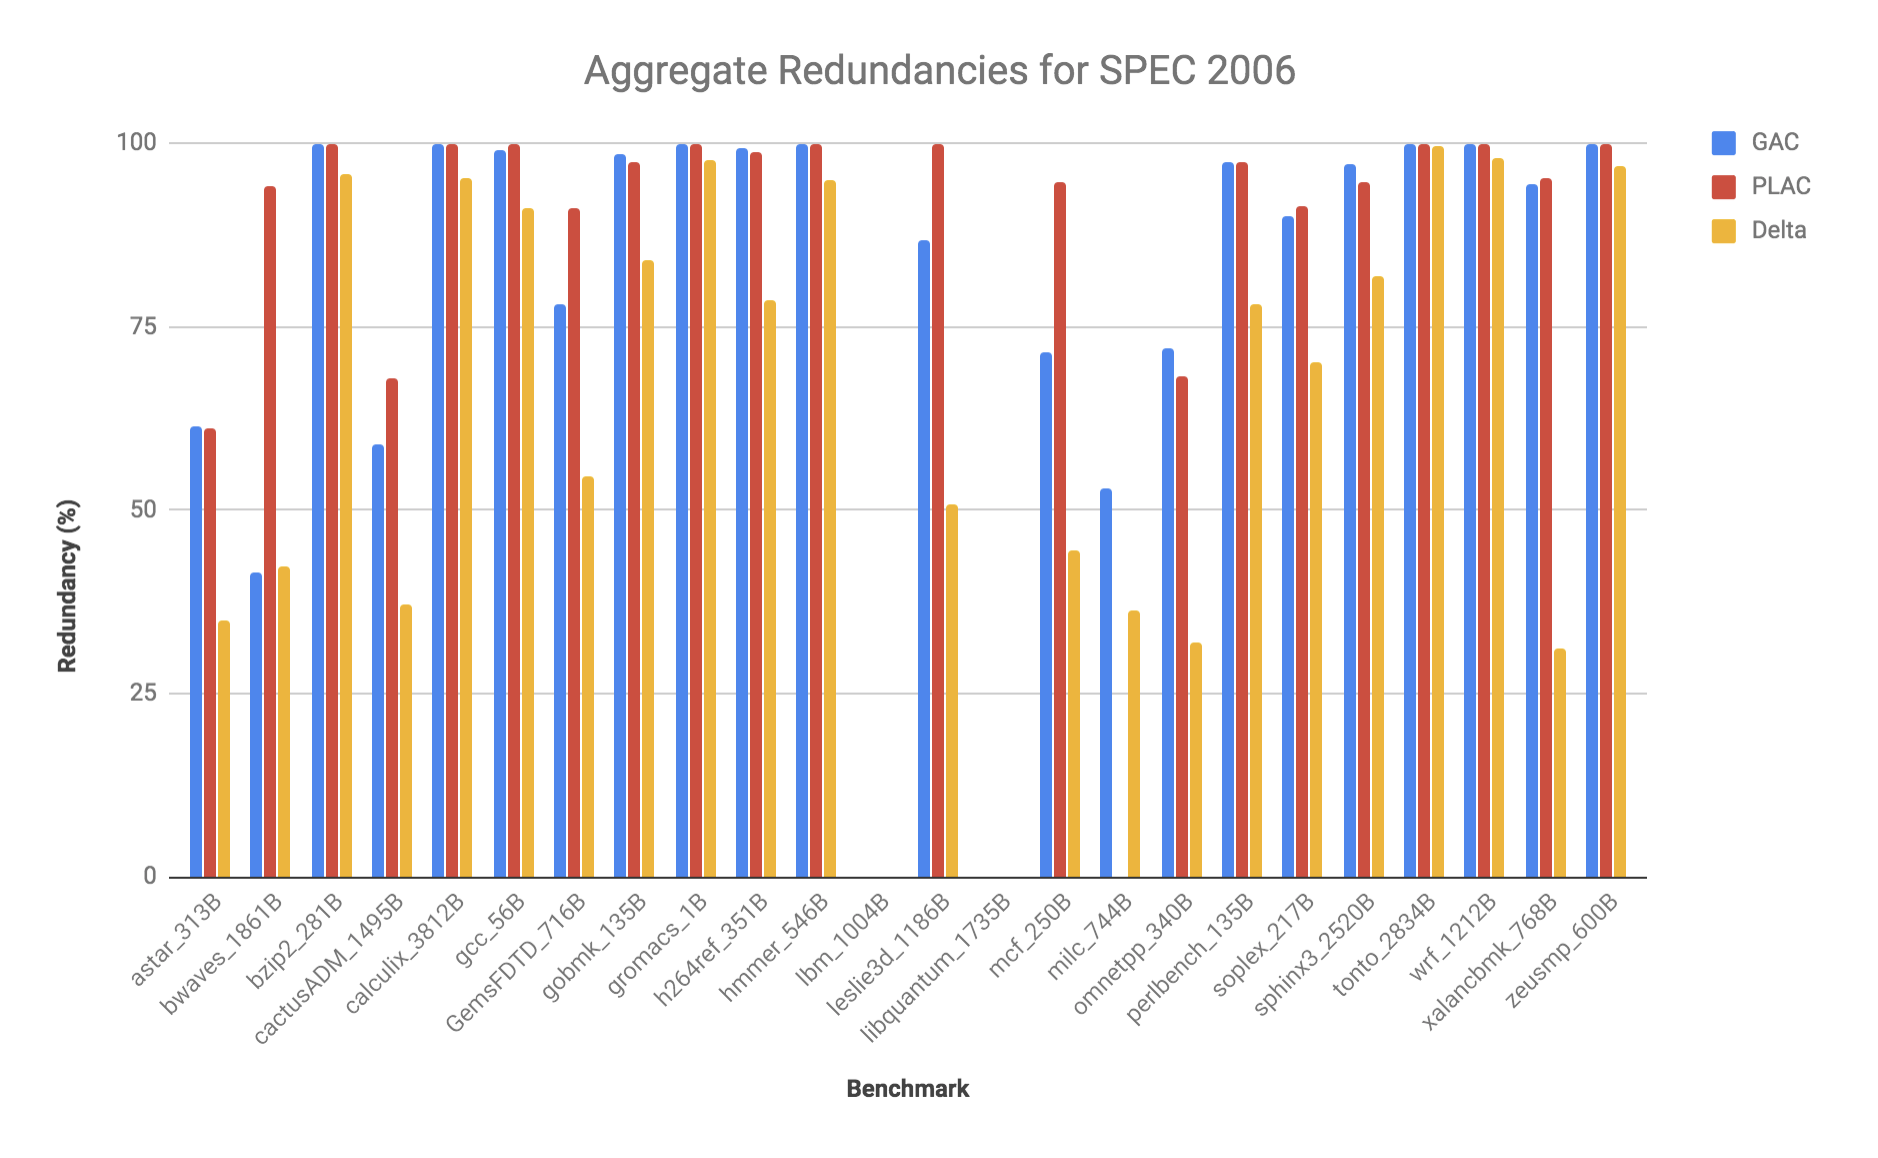
\includegraphics[width=.95\textwidth]{aggregate_redundancy.png}
        \caption{Prefetcher redundancy for SPEC 2006 benchmarks}
        \vspace*{\floatsep}
    \end{figure*}
    
    \begin{figure*}[h] % RUSHI
        \centering
            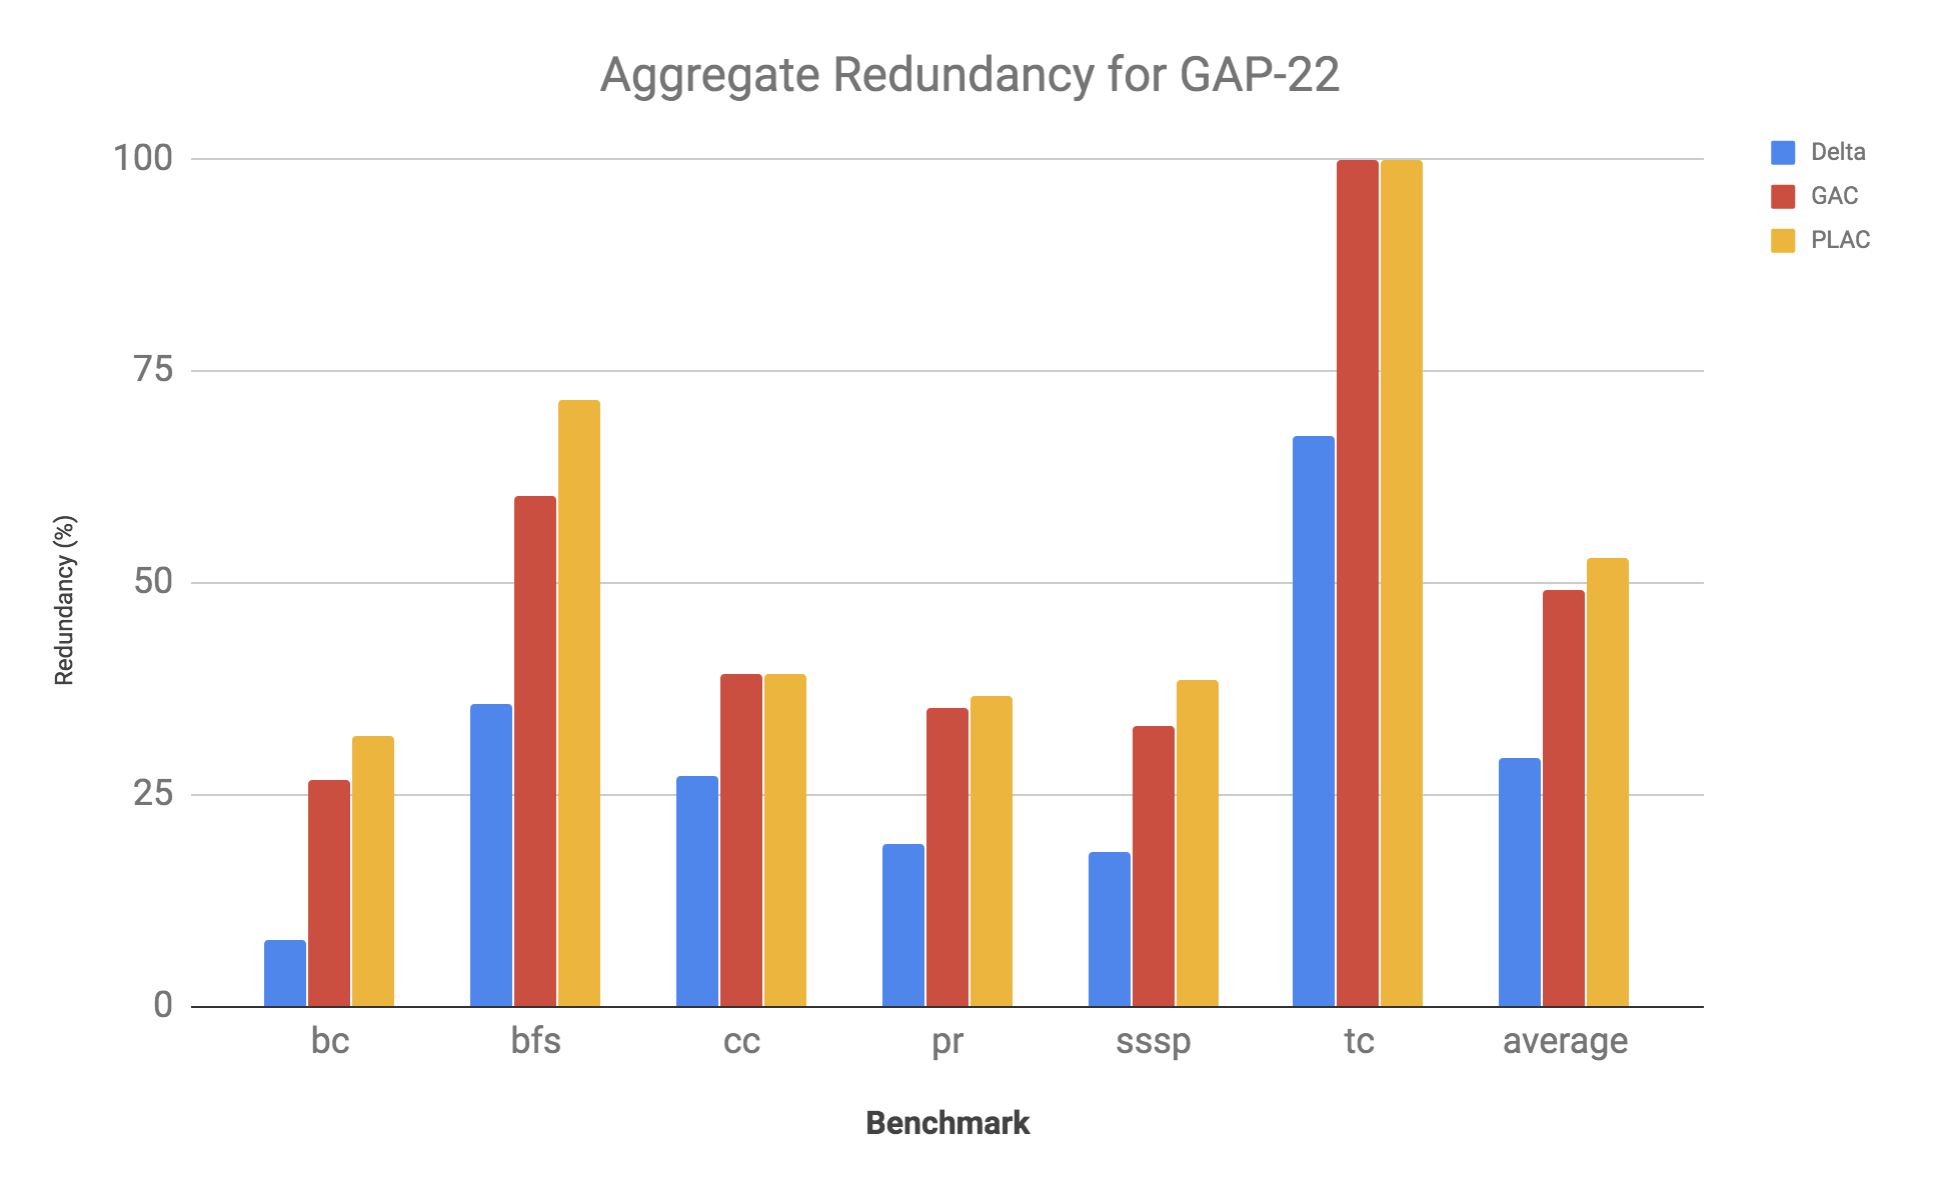
\includegraphics[width=.95\textwidth]{aggregate_redundancy_gap.png}
        \caption{Prefetcher redundancy for GAP-22 benchmarks}
        \vspace*{\floatsep}
        \vspace*{\floatsep}
        \centering
            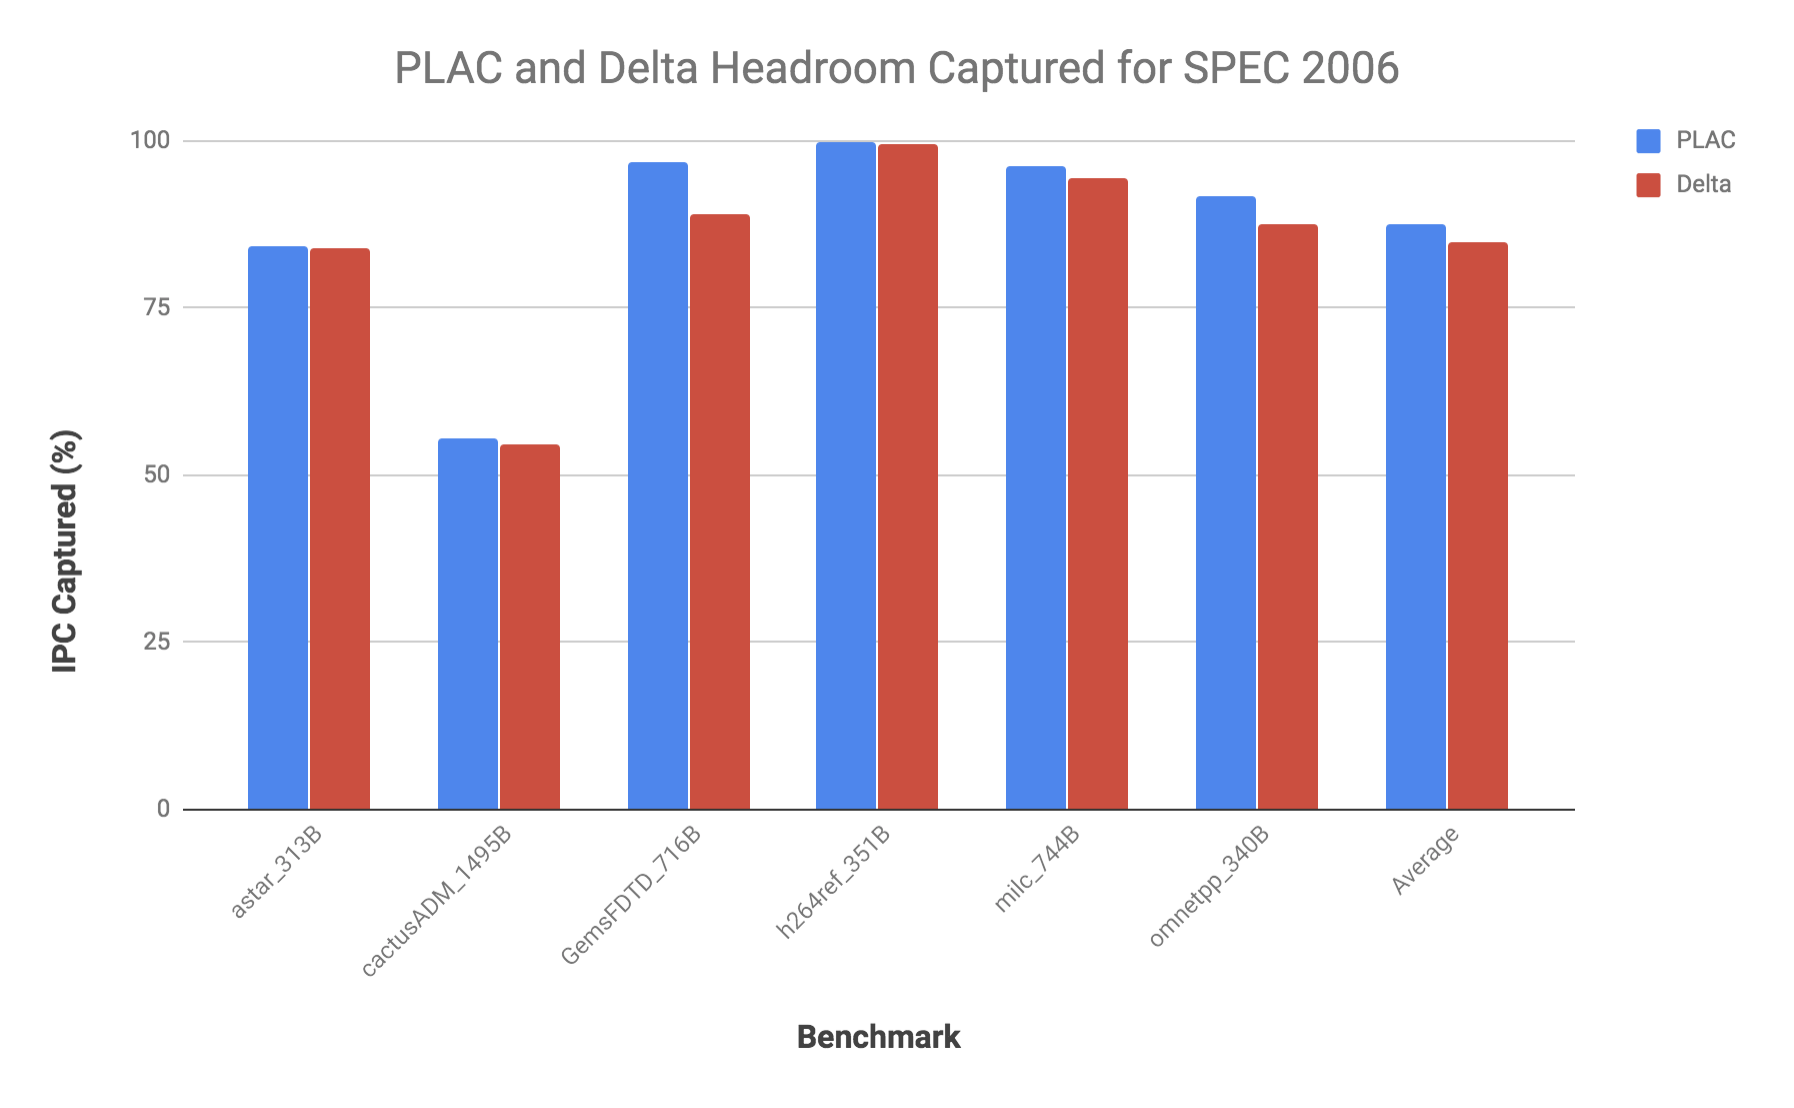
\includegraphics[width=.95\textwidth]{spec_covered.png}
        \caption{Headroom captured for SPEC 2006 benchmarks}
        \vspace*{\floatsep}
    \end{figure*}
    
    \begin{figure*}[h] % RUSHI
        \centering
            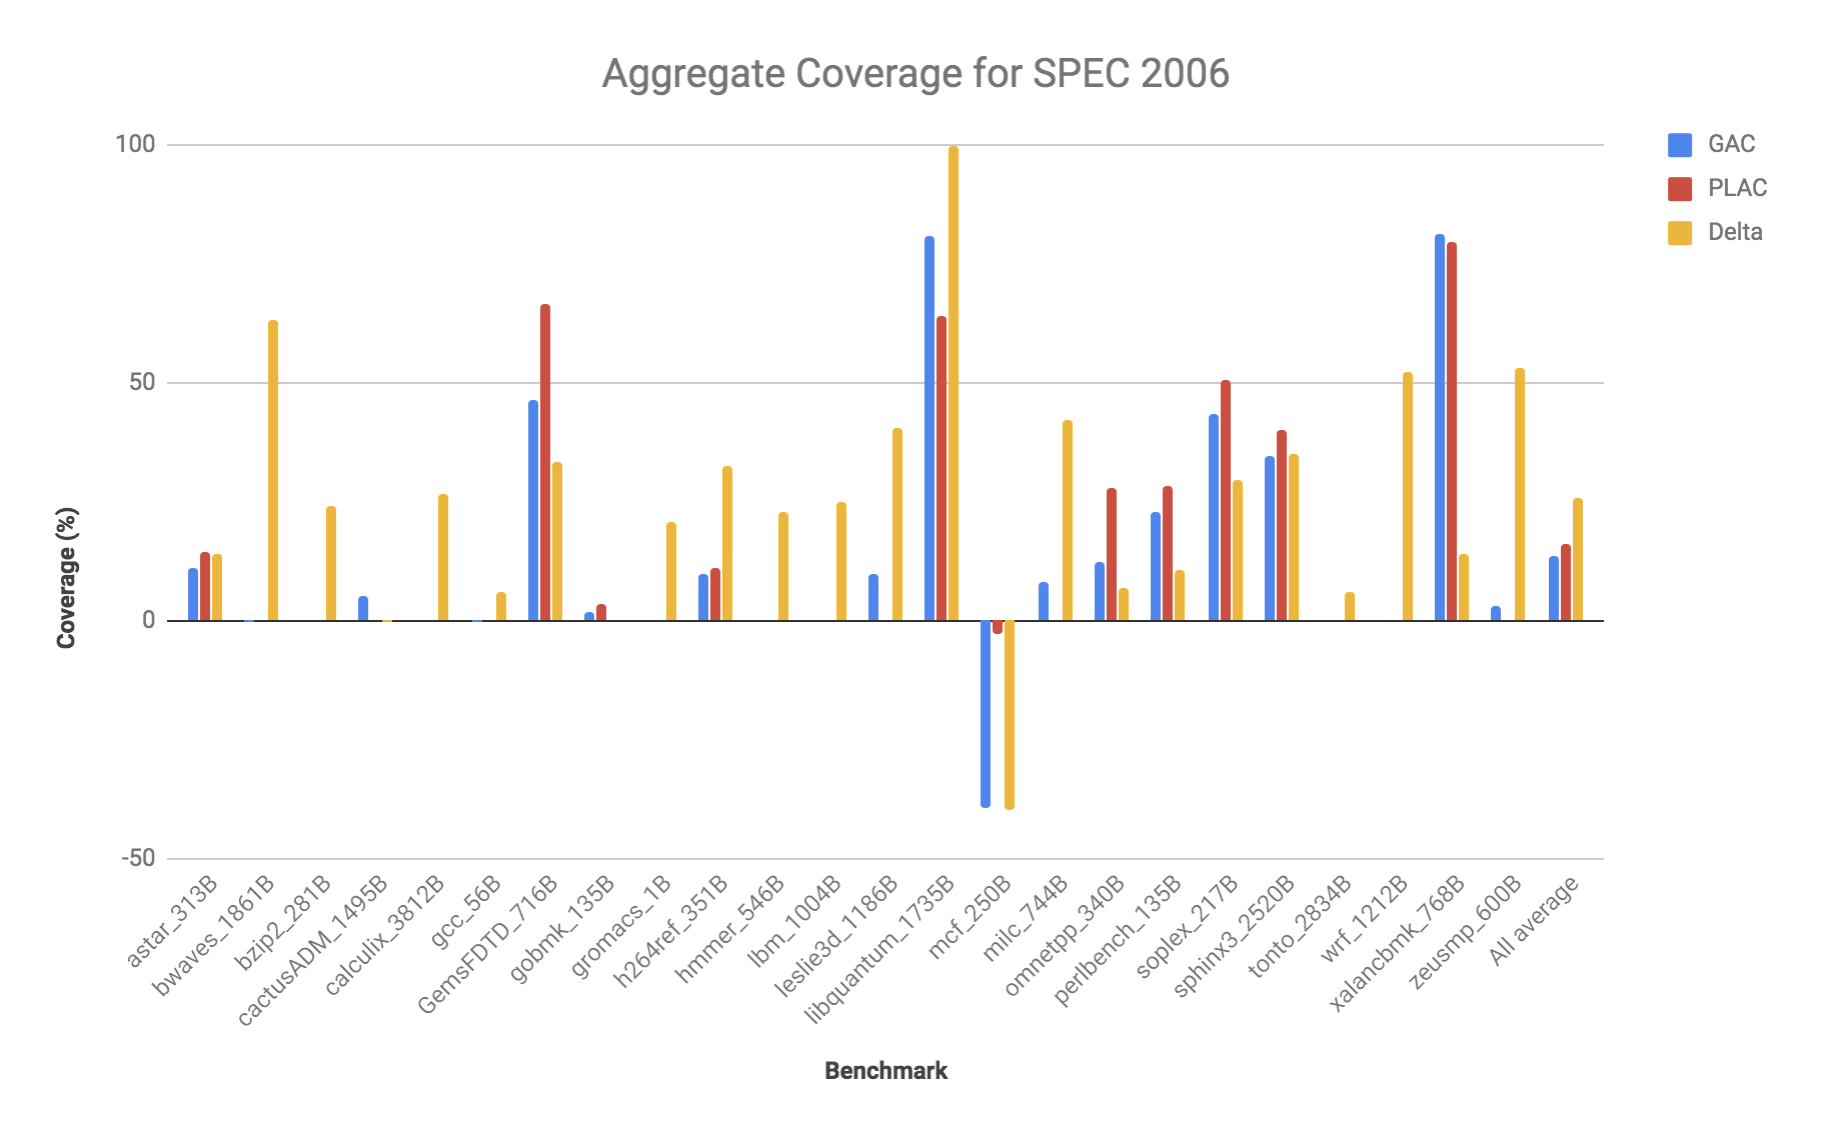
\includegraphics[width=.95\textwidth]{aggregate_coverage.png}
        \caption{Prefetcher coverage for SPEC 2006 benchmarks}
        \vspace*{\floatsep}
        \vspace*{\floatsep}
        \centering
            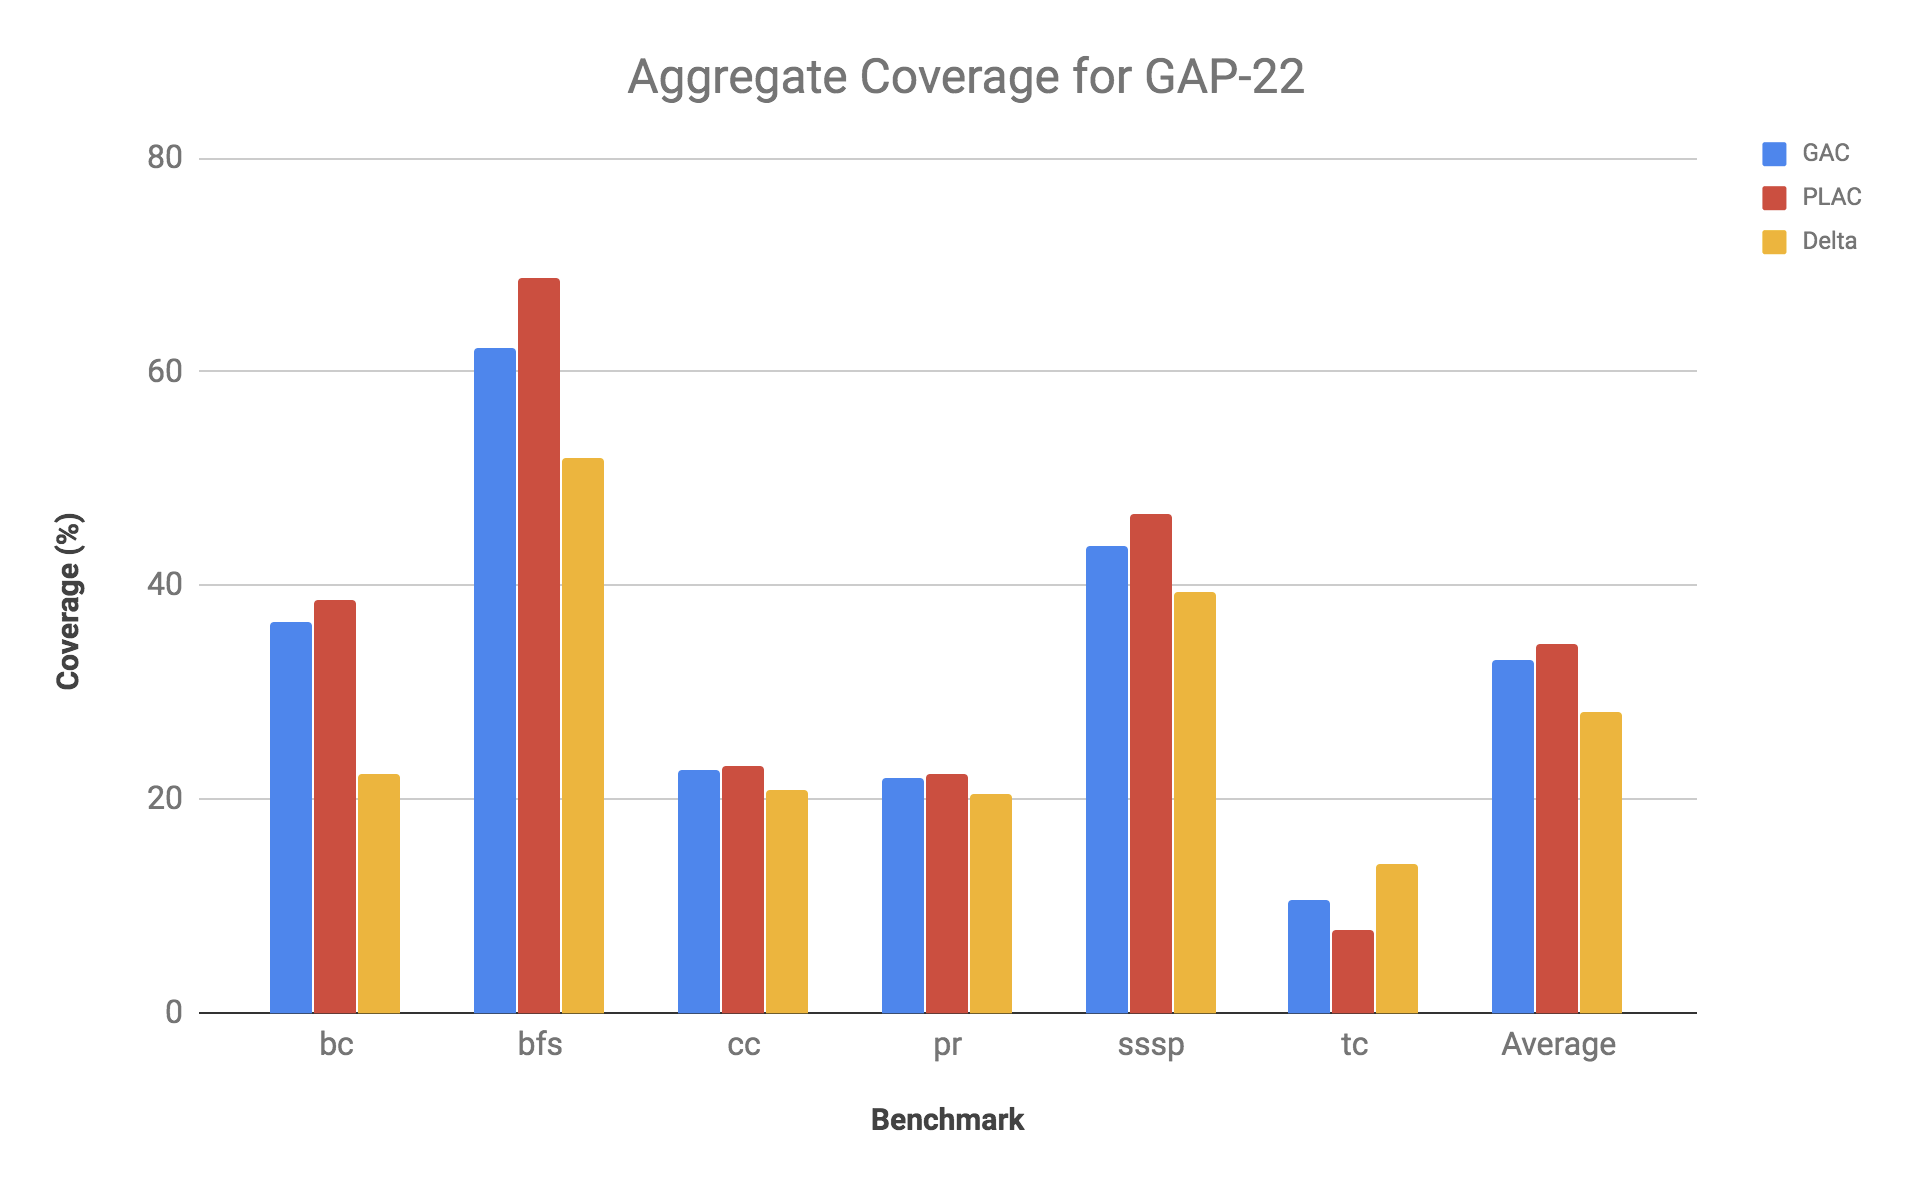
\includegraphics[width=.95\textwidth]{aggregate_coverage_gap22.png}
        \caption{Prefetcher coverage for GAP-22 benchmarks}
    \end{figure*}

\section*{ACKNOWLEDGMENT}

    We would like to thank Calvin Lin, Akanksha Jain, and Matthew Pabst for their guidance and assistance.

\begin{thebibliography}{99}
    \bibitem{c1} Kandiraju, G.b., and A. Sivasubramaniam. “Going the Distance for TLB Prefetching: an Application-Driven Study.” Proceedings 29th Annual International Symposium on Computer Architecture, 2002, doi:10.1109/isca.2002.1003578.
\end{thebibliography}


\end{document}